
%% bare_jrnl.tex
%% V1.4b
%% 2015/08/26
%% by Michael Shell
%% see http://www.michaelshell.org/
%% for current contact information.
%%
%% This is a skeleton file demonstrating the use of IEEEtran.cls
%% (requires IEEEtran.cls version 1.8b or later) with an IEEE
%% journal paper.
%%
%% Support sites:
%% http://www.michaelshell.org/tex/ieeetran/
%% http://www.ctan.org/pkg/ieeetran
%% and
%% http://www.ieee.org/

%%*************************************************************************
%% Legal Notice:
%% This code is offered as-is without any warranty either expressed or
%% implied; without even the implied warranty of MERCHANTABILITY or
%% FITNESS FOR A PARTICULAR PURPOSE! 
%% User assumes all risk.
%% In no event shall the IEEE or any contributor to this code be liable for
%% any damages or losses, including, but not limited to, incidental,
%% consequential, or any other damages, resulting from the use or misuse
%% of any information contained here.
%%
%% All comments are the opinions of their respective authors and are not
%% necessarily endorsed by the IEEE.
%%
%% This work is distributed under the LaTeX Project Public License (LPPL)
%% ( http://www.latex-project.org/ ) version 1.3, and may be freely used,
%% distributed and modified. A copy of the LPPL, version 1.3, is included
%% in the base LaTeX documentation of all distributions of LaTeX released
%% 2003/12/01 or later.
%% Retain all contribution notices and credits.
%% ** Modified files should be clearly indicated as such, including  **
%% ** renaming them and changing author support contact information. **
%%*************************************************************************


% *** Authors should verify (and, if needed, correct) their LaTeX system  ***
% *** with the testflow diagnostic prior to trusting their LaTeX platform ***
% *** with production work. The IEEE's font choices and paper sizes can   ***
% *** trigger bugs that do not appear when using other class files.       ***                          ***
% The testflow support page is at:
% http://www.michaelshell.org/tex/testflow/



%\documentclass[journal,draft,onecolumn]{IEEEtran}
\documentclass[journal]{IEEEtran}
% *** GRAPHICS RELATED PACKAGES ***
%
\ifCLASSINFOpdf
  % \usepackage[pdftex]{graphicx}
  % declare the path(s) where your graphic files are
  % \graphicspath{{../pdf/}{../jpeg/}}
  % and their extensions so you won't have to specify these with
  % every instance of \includegraphics
  % \DeclareGraphicsExtensions{.pdf,.jpeg,.png}
\else
  % or other class option (dvipsone, dvipdf, if not using dvips). graphicx
  % will default to the driver specified in the system graphics.cfg if no
  % driver is specified.
  % \usepackage[dvips]{graphicx}
  % declare the path(s) where your graphic files are
  % \graphicspath{{../eps/}}
  % and their extensions so you won't have to specify these with
  % every instance of \includegraphics
  % \DeclareGraphicsExtensions{.eps}
\fi

\usepackage{hyperref}
\usepackage{stfloats}



%% The amssymb package provides various useful mathematical symbols
\usepackage{amssymb}
\usepackage{framed,multirow}
\usepackage{url,microtype}
\usepackage{mathrsfs,bm} % Notacion de transformadas
\usepackage{amsmath}
\usepackage{amsfonts,eucal}
\usepackage[normalem]{ulem}

\usepackage{epsfig}
\usepackage{epstopdf}
\usepackage{booktabs}
\usepackage{adjustbox}
\usepackage[]{subfigure}
\usepackage{lineno}

\usepackage{tikz}
\usepackage{pgfplots}
%\usetikzlibrary{shadings}
\pgfplotsset{compat=1.16}
%\usetikzlibrary{arrows,shapes,shadows,calc,decorations.pathreplacing,positioning}
%\usetikzlibrary{spy}
\usepgfplotslibrary{fillbetween}

\usepackage{times}
%\usepackage[titletoc,toc,title]{appendix}
\usepackage{natbib}
\usepackage{float}
\usepackage[ruled,linesnumbered]{algorithm2e}
\usepackage{array}
\usepackage{color}
\usepackage[capitalize]{cleveref}
\usepackage{enumerate,multirow}
% \usepackage{lineno}


%%Defining some useful variables 
\providecommand{\promedd}[2]{\mathbb{E}_{#1}\!$\left\{#2\right\}$}% operador de promedio
\providecommand{\ve}[1]{{\bm{#1}}}%
\providecommand{\tr}[1]{{\operatorname{tr}$\left({#1}\right)$}}
\providecommand{\mat}[1]{{\bm{#1}}} %
\providecommand{\var}[1]{${\operatorname{var}}\left\{#1\right\}$}
\newcommand{\Real}{\mathbb{R}}
\newcommand{\N}{\mathbb{N}}
\newcommand{\Z}{\mathbb{Z}}

\DeclareMathOperator{\subconj}{\negthinspace\subset\negthinspace }
\DeclareMathOperator{\en}{\!\,\in\!\,}
\DeclareMathOperator{\igual}{\!\,=\!\,}
\DeclareMathOperator{\dist}{\operatorname{d}}
\DeclareMathOperator{\xx}{\negthickspace\times\negthickspace}
\providecommand{\s}[1]{\negthinspace#1\negthinspace}%

\renewcommand{\refname}{\normalsize References}
\newcommand{\dif}[1]{\mathrm{d}#1}
\newcommand{\Erf}[1]{\mathrm{erf}\left(#1\right)}
\newcommand{\Cov}[1]{\mathrm{cov}\left(#1\right)}
\newcommand{\sign}[1]{\mathrm{sign}(#1)}
\newcommand{\phivec}{\boldsymbol{\phi}}
\newcommand{\muvec}{\boldsymbol{\mu}}
\newcommand{\wfunc}[1]{\textnormal{w}(#1)}
\newcommand{\ex}[1]{\mathbb{E}[#1]}
\providecommand{\ve}[1]{{\mathbf{#1}}}

\DeclareMathOperator{\vecO}{vec} % vec operator
\providecommand{\mat}[1]{{\mathbf{#1}}}
\DeclareMathOperator{\cov}{cov} % Operator for the covariance
\DeclareMathOperator{\KL}{KL} % Operator for the KL divergence
\newcommand{\boldk}{\mathbf{k}} % kernel or covariance
\newcommand{\boldt}{\mathbf{t}} % kernel or covariance
\newcommand{\boldK}{\mathbf{K}} % kernel or covariance
\newcommand{\boldf}{\mathbf{f}} % outputs without noise
\newcommand{\boldB}{\mathbf{B}} % coregionalization matrix
\newcommand{\boldA}{\mathbf{A}} % matrix of coeffcients a_{qi}^r
\newcommand{\boldc}{\mathbf{c}} % matrix of coeffcients a_{qi}^r
\newcommand{\boldu}{\mathbf{u}} % vector for latent function
\newcommand{\bolda}{\mathbf{a}}
\newcommand{\boldm}{\mathbf{m}}
\newcommand{\boldv}{\mathbf{v}}
\newcommand{\boldV}{\mathbf{V}}
\newcommand{\boldW}{\mathbf{W}}
\newcommand{\boldY}{\mathbf{Y}}
\newcommand{\boldy}{\mathbf{y}}
\newcommand{\boldZ}{\mathbf{Z}}
\newcommand{\boldz}{\mathbf{z}}
\newcommand{\boldAtilde}{\mathbf{\widetilde{A}}}
\newcommand{\eye}{\mathbf{I}}   % identity matrix
\newcommand{\boldI}{\mathbf{I}} % identity matrix
\newcommand{\boldUpsi}{\bm{\Upsilon}}
\newcommand{\boldH}{\mathbf{H}} % The whole set of lag vectors
\newcommand{\inputSpace}{\mathcal{X}} % The input space
\newcommand{\params}{\bm{\theta}} % Parameters of LMC model
\newcommand{\veC}{\textbf{\hspace{-0.001in}:}} % Simplified version of the vec operator (vec = :)
\newcommand{\preci}{\mathbf{P}}% Precision for the Gaussians
\newcommand{\dataset}{{\cal D}} % dataset
\newcommand{\fracpartial}[2]{\frac{\partial #1}{\partial  #2}} % Fraction for partial derivatives
\newcommand{\gauss}{\mathcal{N}} % Gaussian density
\newcommand{\bolds}{\mathbf{s}}


\newcommand\redsout{\bgroup\markoverwith{\textcolor{red}{\rule[0.5ex]{2pt}{0.4pt}}}\ULon}
\providecommand{\roj}[1]{\textcolor{red}{\uwave{#1}}}
\providecommand{\ver}[1]{\textcolor{green}{\uwave{#1}}}
\providecommand{\gc}[1]{\textcolor{darkgray}{\uwave{#1}}}
\providecommand{\am}[1]{\textcolor[rgb]{0.1,0.5,0.0}{\upshape{#1}}}
% Leave a blank line between paragraphs instead of using \\

%Comments
\providecommand{\am}[1]{\textcolor[rgb]{0.1,0.5,0.0}{\upshape{#1}}}

\newcolumntype{C}[1]{>{\centering\let\newline\\\arraybackslash\hspace{0pt}}m{#1}}

\usepackage{pifont}% http://ctan.org/pkg/pifont
\newcommand{\cmark}{\ding{51}}%
\newcommand{\xmark}{\ding{55}}%
\usetikzlibrary{bayesnet}

% correct bad hyphenation here
\hyphenation{op-tical net-works semi-conduc-tor}

\newcommand{\comment}[2]{{\color{blue}#1} {\color{red}#2}}
% \AtBeginEnvironment{appendices}{\crefalias{section}{appendix}}
\begin{document}
%
% paper title
% Titles are generally capitalized except for words such as a, an, and, as,
% at, but, by, for, in, nor, of, on, or, the, to and up, which are usually
% not capitalized unless they are the first or last word of the title.
% Linebreaks \\ can be used within to get better formatting as desired.
% Do not put math or special symbols in the title.
\title{Correlated Chained Gaussian Processes with Multiple Annotators}
%
%
% author names and IEEE memberships
% note positions of commas and nonbreaking spaces ( ~ ) LaTeX will not break
% a structure at a ~ so this keeps an author's name from being broken across
% two lines.
% use \thanks{} to gain access to the first footnote area
% a separate \thanks must be used for each paragraph as LaTeX2e's \thanks
% was not built to handle multiple paragraphs
%

\author{J. Gil-Gonz\'alez,
        J. Giraldo,
        A. \'Alvarez-Meza, A. Orozco-Guti\'errez,  and~M.~A.~\'Alvarez% <-this % stops a space
\thanks{J. Gil-Gonz\'alez and A. Orozco are with the Universidad Tecnol\'ogica de Pereira, Colombia, 660003, e-mail:\{jugil,aaog\}@utp.edu.co}% <-this % stops a space
\thanks{J. Giraldo and M. A.\'Alvarez are with the University of Sheffield, UK. email: \{jjgiraldogutierrez1,mauricio.alvarez\}@sheffield.ac.uk}% <-this % stops a space
\thanks{A. \'Alvarez is with the Universidad Nacional de Colombia sede Manizales, 170001, Colombia. email: amalvarezme@unal.edu.co}}
%\thanks{Manuscript received April 19, 2005; revised August 26, 2015.}}

% note the % following the last \IEEEmembership and also \thanks - 
% these prevent an unwanted space from occurring between the last author name
% and the end of the author line. i.e., if you had this:
% 
% \author{....lastname \thanks{...} \thanks{...} }
%                     ^------------^------------^----Do not want these spaces!
%
% a space would be appended to the last name and could cause every name on that
% line to be shifted left slightly. This is one of those "LaTeX things". For
% instance, "\textbf{A} \textbf{B}" will typeset as "A B" not "AB". To get
% "AB" then you have to do: "\textbf{A}\textbf{B}"
% \thanks is no different in this regard, so shield the last } of each \thanks
% that ends a line with a % and do not let a space in before the next \thanks.
% Spaces after \IEEEmembership other than the last one are OK (and needed) as
% you are supposed to have spaces between the names. For what it is worth,
% this is a minor point as most people would not even notice if the said evil
% space somehow managed to creep in.



% The paper headers
\markboth{Journal of \LaTeX\ Class Files,~Vol.~14, No.~8, August~2015}%
{Shell \MakeLowercase{\textit{et al.}}: Bare Demo of IEEEtran.cls for IEEE Journals}
% The only time the second header will appear is for the odd numbered pages
% after the title page when using the twoside option.
% 
% *** Note that you probably will NOT want to include the author's ***
% *** name in the headers of peer review papers.                   ***
% You can use \ifCLASSOPTIONpeerreview for conditional compilation here if
% you desire.




% If you want to put a publisher's ID mark on the page you can do it like
% this:
%\IEEEpubid{0000--0000/00\$00.00~\copyright~2015 IEEE}
% Remember, if you use this you must call \IEEEpubidadjcol in the second
% column for its text to clear the IEEEpubid mark.



% use for special paper notices
%\IEEEspecialpapernotice{(Invited Paper)}




% make the title area
\maketitle


\linenumbers

% As a general rule, do not put math, special symbols or citations
% in the abstract or keywords.
\begin{abstract}
 The labeling process within a supervised learning task is usually carried out by an expert, which provides the ground truth (gold standard) for each sample. However, in many real-world applications, we typically have access to annotations provided by crowds holding different and unknown expertise levels. Learning from crowds intends to configure machine learning paradigms in the presence of multi-labelers, residing on two key assumptions: the labeler’s performance does not depend on the input space, and independence among the annotators is imposed. Here, we propose the correlated chained Gaussian processes from multiple annotators--(CCGPMA) approach, which models each annotator's performance as a function of the input space and exploits the correlations among experts. Experimental results associated with regression and classification tasks show that our CCGPMA achieves suitable performances from inconsistent labelers, even if the gold standard is not available.
\end{abstract}

% Note that keywords are not normally used for peerreview papers.
\begin{IEEEkeywords}
Multiple annotators, Correlated Chained Gaussian Processes, Classification, Regression.
\end{IEEEkeywords}

% For peer review papers, you can put extra information on the cover
% page as needed:
% \ifCLASSOPTIONpeerreview
% \begin{center} \bfseries EDICS Category: 3-BBND \end{center}
% \fi
%
% For peerreview papers, this IEEEtran command inserts a page break and
% creates the second title. It will be ignored for other modes.
\IEEEpeerreviewmaketitle



\section{Introduction}

\IEEEPARstart{S}{upervised} learning requires that a domain expert labels the instances to built the gold standard (ground truth)~\cite{zhang2019crowdsourced}. Yet, the experts are scarce, or their time is expensive, not mentioning that the labeling task is tedious and
time-consuming~\cite{liu2020truth}. As an alternative, the labeling is distributed through multiple
heterogeneous annotators, who annotate part of the whole dataset by providing their
version of the hidden ground truth~\cite{kara2015modeling}.
Recently, crowdsourcing platforms, i.e., Amazon Mechanical Turk-- (AMT)\footnote{https://www.mturk.com/}, have been introduced to capture labels from multiple sources on large datasets efficiently. The attractiveness of these platforms lies in that, at a low cost, it is possible to obtain suitable quality labels. Indeed, in some cases, such a labeling process can compete with those provided by
experts~\cite{snow2008cheap}. However, in such an multi-labelers scenario, each instance is matched with multiple annotations provided by different
sources with unknown and diverse expertise, being difficult to apply traditional supervised learning
algorithms~\cite{tao2018domain}. In this sense, \emph{learning from crowds} has been introduced as a general framework from two main perspectives: to fit the labels from multiple annotators or to adapt the
supervised learning algorithms~\cite{rizos2020average}. 

The first approach is known in the literature as ``label aggregation''
or ``truth inference'', comprising the computation of a single hard
label per sample as an estimation of the ground truth. The
hard labels are then used to feed a standard supervised learning
algorithm~\cite{morales2019scalable}. The straightforward method is the so-called majority voting--(MV), and it has been used in
different multi-labeler problems due to its
simplicity~\cite{zhang2014imbalanced}. Still, MV assumes homogeneity
in annotators' reliability, which is hardly feasible in real
applications, e.g., experts vs. spammers. Furthermore, the consensus
is profoundly impacted by incorrect labels and
outliers~\cite{kara2015modeling}. Conversely, more elaborated models
have been considered to improve the estimation of the correct tag through the well-known Expectation-Maximization--(EM) framework and by facing the imbalanced labeling issue~\cite{dawid1979maximum,zhang2014imbalanced}.

The second approach jointly trains the supervised learning algorithm and models the annotators' behavior. It has been shown that such strategies lead to better performance compared to the ones belonging to label
aggregation. Thus, the features used to train the learning algorithm
provide valuable information to puzzle out the ground
truth~\cite{ruiz2019learning}. The most representative work in this area is exposed in \cite{raykar2010learning}, which offers an EM-based framework to learn the parameters of a logistic regression classifier and model the annotators' behavior by computing their sensitivities and specificities. In fact, such a technique has inspired several models
in the context of multi-labelers scenarios, including binary
classification~\cite{rodrigues2014gaussian,ruiz2019learning},
multi-class discrimination~\cite{morales2019scalable,gonzalez2015automatic}, regression~\cite{groot2011learning,rodrigues2017learning}, and sequence
labeling~\cite{rodrigues2014sequence}. Furthermore, some works have addressed the multi-labeler problem using deep learning approaches to design an extra layer coding the
annotators' information~\cite{albarqouni2016aggnet,rodrigues2018deep,guan2018said}. 

Two main issues are still unsolved in the context of learning from crowds~\cite{g2019machine}: we need to code the relationships between the input
features and the labelers' performance while revealing relevant annotators' interdependencies. In general,  the annotators' behavior is parametrized through a homogeneous constraint across the input samples. The latter assumption is not correct since an expert makes decisions based not only on his/her expertise but also on the features observed from raw data ~\cite{raykar2010learning}. Besides, it is
widespread to consider independence in the annotators' labels, aiming
to reduce the complexity of the model~\cite{venanzi2014community}, or
based on the fact that it is plausible to guarantee that each labeler
performs the annotation process
individually~\cite{tang2019leveraging}. However, this assumption is
not true since there may exist correlations among the
annotators \cite{zhang2011learning}. For example, if the sources are
humans, the independence assumption is hardly feasible because
knowledge is a social construction; then, people's decisions will be
correlated because they share information or belong to a particular school of
thought~\cite{surowiecki2005wisdom,hahn2018communication}. Now, if we consider that the sources are algorithms, where some of them gather the same math principle, there likely exists a
correlation in their labels~\cite{zhu2019unsupervised}. 

In this work, we propose a probabilistic model, named the correlated chained Gaussian Processes for multiple annotators--(CCGPMA), to jointly build a prediction algorithm applicable to regression and classification tasks. CCGPMA is based on the chained GPs model--(CGP) \cite{saul2016chained}, which is a Multi-GPs framework where the
parameters of an arbitrary likelihood function are modeled with
multiple independent GPs (one GP prior per parameter). Unlike CGP, we consider that multiple correlated GPs model the likelihood's parameters. For doing so, we take as a basis the ideas from a Multi-output GP--(MOGP) regression~\cite{alvarez2012kernels}, where each output is coded as a weighted sum of shared latent functions via a semi-parametric latent factor model--(SLFM)~\cite{teh2005semiparametric}. In contrast to the MOGP, we do not have multiple outputs but multiple functions chained to the given likelihood parameters. From the multiple annotators' point of view, the likelihood parameters are related to the labelers' behavior; thereby, CCGPMA models the labelers' behavior as a function of the input features while also taking into account annotators' interdependencies. Moreover, our proposal is based on the so-called inducing variables framework~\cite{alvarez2010efficient}, in combination with stochastic variational inference~\cite{hoffman2013stochastic}. To the best of our knowledge, this is the first attempt to build a probabilistic approach to model the labelers' behavior as a function of the input features while also considering annotators' interdependencies. Achieved results, using both simulated and real-world data, show how our method can deal with both regression and classification problems from multi-labelers data.

The remainder is organized as follows. Section 2 exposes the related
work and the main contributions of the proposal. Section 3 describes the
methods. Sections 4 and 5 present the experiments and discuss the
results. Finally, Section 6 outlines the conclusions and future work.

\section{Related work and main contributions}

Most of the learning from crowds-based methods aim to model the annotators' behavior based on the accuracy~\cite{rodrigues2013learning}, the confusion matrix~\cite{gonzalez2015automatic}, the error variance~\cite{raykar2010learning}, and the bias~\cite{rodrigues2017learning}. Concerning this, the expert parameters are modeled as fixed points~\cite{rodrigues2014gaussian}, or as random variables, where it is considered that such parameters are homogeneous across the input data~\cite{morales2019scalable}. 

The first attempt to analyze the relationship between the annotators' parameters and the input features is the work in~\cite{zhang2011learning}. The authors propose an approach for binary classification with multiple labelers, where the input data is represented by a defined cluster using a Gaussian Mixture Model--(GMM). The approach assumes that the annotators
exhibit a particular performance measured in terms of sensitivity and
specificity for each group. However, the model does not consider the information from multiple experts as an input for the GMM, yielding variations in the labelers' parameters. Similarly, in \cite{yan2014learning}, the authors propose a binary classification algorithm that employs two probability models to code the annotators' performance as a function of the input space, namely a
Bernoulli and a Gaussian distribution. The parameters of these
distributions are computed via Logistic regression. Nonetheless, a linear dependence between the labeler expertise and the input space is assumed, which may not be appropriate because of the data structure's nonlinearities. For example, if we consider online annotators assessing some documents, they may have different labeling accuracy. Such differences may rely on whether they are more familiar with some issues than other~\cite{wang2016bi}. Authors in \cite{xiao2013learning} offer a GP-based regression with multiple annotators. An additional GP models the annotators' parameters as a nonlinear function of the input space. Yet, the inference is carried out based on maximum a posteriori (MAP), without including uncertainty parameters.

On the other hand, it has been shown that the relaxation of the  annotators' independence restriction can improve the ground truth estimation~\cite{zhang2011learning,g2019machine}. To the best of our knowledge, only two works address such an issue. First, the authors in \cite{zhu2019unsupervised} describe an approach to deal with regression problems, where the labelers' behavior is modeled using a multivariate Gaussian distribution. Thus, the annotators' interdependencies are coded in the covariance matrix. Further, in \cite{gil2018learning}, the authors propose a binary classification method based on a weighted combination of classifiers. In turn, the weights are estimated by using a kernel alignment-based algorithm considering dependencies among the labelers. 

Here, we propose a GPs-based framework to face classification and regression settings with multiple annotators. Our proposal follows the line of the works in~\cite{rodrigues2014gaussian,groot2011learning,ruiz2019learning,morales2019scalable,morales2019scalable1} in the sense that we are modeling the unknown ground truth trough a GP prior. However, while such approaches code the annotators' parameters as fixed points \cite{rodrigues2014gaussian,groot2011learning}; or as
random variable \cite{ruiz2019learning,morales2019scalable,morales2019scalable1}; we model them as random processes to take into account dependencies between the input space and the labelers' behavior. Besides, our CCGPMA shares some similarities with the works in~\cite{yan2014learning,xiao2013learning}, because we aim to model the dependencies between the input features and the labelers' performance. Our method is also similar to the works in~\cite{zhu2019unsupervised,gil2018learning}, because they assume dependencies in the annotators' labels. In contrast, CCGPMA is the only one that includes both assumptions to code the annotators' behavior. Of note, we highlight that our proposal codes inconsistent
annotations, being robust against outliers.  Namely, CCGPMA can estimate the annotators'
performance for every region in the input space; meanwhile, state-of-the-art techniques assess it based on a conventional averaging~\cite{rodrigues2017learning,morales2019scalable,ruiz2019learning}. \cref{tab:SOA} summarizes the key insights of our CCGPMA and state-of-the-art approaches.


\begin{table*}[!tb]
	\centering
	\caption{Survey of relevant supervised learning models devoted to multiple annotators.}
	\resizebox{1\linewidth}{!}{
		\begin{tabular}{C{5cm}C{4cm}C{2.5cm}C{2cm}C{2cm}C{2cm}}\toprule
			Source & Data type & Type of model & Modeling the annotator’s expertise & Expertise as a function of the input space & Modeling the annotators' interdependencies 
            \\\midrule
            \textit{Raykar et al., 2010} \cite{raykar2010learning} & Regression-Binary-Categorical & Probabilistic & \cmark & \xmark & \xmark\\
            \textit{Zhang and Obradovic, 2011} \cite{zhang2011learning} & Binary & Probabilistic & \cmark & \cmark & \xmark\\
            \textit{Xiao et al., 2013} \cite{xiao2013learning} & Regression & Probabilistic & \cmark & \cmark & \xmark\\
            \textit{Yan et al., 2014} \cite{yan2014learning} & Binary & Probabilistic & \cmark & \cmark & \xmark\\
            \textit{Wang and Bi, 2016} \cite{wang2016bi}& Binary & Deterministic & \cmark & \cmark & \xmark\\
            \textit{Rodrigues et al., 2017} \cite{rodrigues2017learning} & Regression-Binary-Categorical & Probabilistic & \cmark & \xmark & \xmark\\
            \textit{Gil-Gonzalez et al., 2018} \cite{gil2018learning} & Binary & Deterministic & \cmark & \xmark & \cmark\\
            \textit{Hua et al., 2018} \cite{hua2018collaborative} & Binary-Categorical & Deterministic & \cmark & \xmark & \xmark\\
            \textit{Ruiz et al., 2019} \cite{ruiz2019learning} & Binary & Probabilistic & \cmark & \xmark & \xmark\\
            \textit{Morales- ́Alvarez et al., 2019} \cite{morales2019scalable} & Binary & Probabilistic & \cmark & \xmark & \xmark\\
            \textit{Zhu et al., 2019} \cite{zhu2019unsupervised} & Regression & Probabilistic & \cmark & \xmark & \cmark\\
            \textbf{Proposal-(CCGPMA)} & Regression-Binary-Categorical & Probabilistic & \cmark & \cmark & \cmark\\\bottomrule
	\end{tabular}} 
	\label{tab:SOA}
\end{table*}



\section{Methods}\label{sec:methods}

\subsection{Correlated chained Gaussian processes}

Let us consider an input-output dataset $\dataset\igual\{\ve{X}\s{\in}\mathcal{X},\ve{y}\s{\in}\mathcal{Y}\},$ where $\mat{X}\igual \left\{\ve{x}_n\s{\in}\mathcal{X}\!\subseteq\!\Real^P\right\}_{n=1}^{N}$ and $\mat{y}\igual\left\{y_n\s{\in} \mathcal{Y}\right\}_{n=1}^{N}$. In turn, let a GP be a collection of random variables $f(\ve{x})$ indexed by the input samples $\ve{x}\en \mathcal{X}$ holding a joint multivariate Gaussian distribution~\cite{rasmussen2006gaussian}. A GP is defined by its mean $m(\ve{x})\igual \ex{f(\ve{x})}$ (we consider $m(\ve{x})\igual0$) and covariance function $\kappa_f(\ve{x}, \ve{x^{\prime}})\igual \ex{(f(\ve{x})-m(\ve{x}))(f(\ve{x'})-m(\ve{x'}))}$, where $\kappa_f\s{:}\mathcal{X}\times\mathcal{X}\s{\to}\Real$ is a given kernel function and $\ve{x}^\prime\en\mathcal{X}$, yielding:

\begin{align} f(\ve{x}) \sim \mathcal{GP} (0, \kappa_f(\ve{x}, \ve{x^{\prime}})).
\end{align}
If we consider the finite set of inputs in $\mat{X}$, then $\ve{f}\igual\left[f(\ve{x}_1), \dots , f(\ve{x}_N)\right]^{\top}\en \Real^{N}$ is drawn for a multivariate Gaussian distribution $\ve{f} \sim \gauss(\ve{f}|\ve{0},\mat{K}_{\ve{f}\ve{f}})$, where $\mat{K}_{\ve{f}\ve{f}}\en\Real^{N\times N}$ is the covariance matrix formed by the evaluation of $\kappa_f(\cdot,\cdot)$ over the input set $\mat{X}$.
Accordingly, using GPs for modeling the input-output data collection $\dataset$ consists of constructing a joint distribution between a given likelihood function and one or multiple GP-based priors. To code each likelihood parameter as a random process, we employ the so-called chained GP--(CGP) that attaches such parameters to multiple independent GP priors, as follows~\cite{saul2016chained}:

\begin{align}
    \notag p(\ve{y}, \hat{\ve{f}}| \mat{X}) =& \prod_{n=1}^{N}p(y_n|\theta_1(\ve{x}_n),\dots , \theta_J(\ve{x}_n))\times \cdots \\
    &\cdots \times \prod_{j=1}^{J}\gauss(\ve{f}_j|\ve{0},\mat{K}_{\ve{f}_j\ve{f}_j})\label{eq:CGP},
\end{align}
where each $\{\theta_j(\ve{x}) \en \mathcal{M}_j\}_{j=1}^{J}$ represents the likelihood's parameters, being $J\en\mathbb{N}$ the number of parameters to represent the likelihood. Besides, each $\theta_j(\ve{x})$ holds a non-linear mapping from a GP prior, e.g., $\theta_j(\ve{x})\igual h_j(f_j(\ve{x}))$, where $h_j\s{:}\Real\to \mathcal{M}_j$ is a deterministic function that maps each latent function--(LF) $f_j(\ve{x}),$ to the appropriate domain $\mathcal{M}_j$. Moreover, $\ve{f}_j\igual\left[f_j(\ve{x}_1), \dots , f_j(\ve{x}_N)\right]^{\top}\en\Real^{N}$ is a LF vector that follows a GP prior, and $\hat{\ve{f}}\igual\left[\ve{f}_1, \dots , \ve{f}_J\right]^{\top}\en \Real^{NJ}$. $\mat{K}_{\ve{f}_j\ve{f}_j} \en\Real^{N\times N}$ is the covariance matrix belonging to the $j$-th GP prior, which is computed based on the kernel function  $\kappa_{j}\s{:}\mathcal{X}\times\mathcal{X}\s{\to}\Real$.

From the above, we note that the CGP model assumes independence between priors, thereby lacking a correlation structure between GPs. The latter is unrealistic because one would expect the parameters to be correlated. Therefore, we introduce the correlated chained GPs--(CCGP) to model correlations between the GP latent functions, which are supposed to be generated from a semi-parametric latent factor model--(SLFM)~\cite{teh2005semiparametric}:

\begin{align}
\label{eq:SLFM}
f_j(\ve{x}_n) = \sum_{q=1}^{Q} w_{j,q} \mu_{q}(\ve{x}_n),
\end{align}
where $f_j\s{:}\mathcal{X}\s{\to}\Real$ is an LF, ${k}_q\s{:}\mathcal{X}{\times}\mathcal{X}\s{\to}\Real$ is a kernel function, $\mu_q(\cdot) \sim \mathcal{GP}(0,{k}_q(\cdot, \cdot))$, and $w_{j,q}\en\Real$ is a combination coefficient ($Q\en\mathbb{N}$). Here, each LF is chained to the likelihood's parameters to extend the joint distribution in \cref{eq:CGP} as follows:

\begin{align}
p(\ve{y},\hat{\ve{f}},\ve{u}|\mat{X})=p(\ve{y}|\bm{\theta}) \prod_{j=1}^{J}p(\ve{f}_j|{\ve{u}})p({\ve{u}}),
\end{align} 
where $\bm{\theta}\igual[\bm{\theta}_1,\dots ,\bm{\theta}_J]^{\top}\en\Real^{NJ}$ holds the model's parameters and $\bm{\theta}_j\igual[\theta_j(\ve{x}_1),\dots ,\theta_j(\ve{x}_N)]^{\top}\en\Real^{N}$ relates the $j$-th parameter with the input space. Our CCGP employs the inducing variables-based method for sparse approximations of GPs~\cite{hensman2015scalable}. For each $\mu_q(\cdot)$, we introduce a set of $M\s{\leq}N$ ``pseudo variables'' $\ve{u}_ q\igual [\mu_q(\ve{z}_1^q), \dots , \mu_q(\ve{z}_M^q)]^{\top}\en \Real^{M}$ through evaluations of $\mu_q(\cdot)$ at unknown locations $\mat{Z}_q \igual [\ve{z}_1^q, \dots , \ve{z}_M^q]\en \Real^{M\times P}$. Note that ${\ve{u}} \igual \left[\ve{u}_1^{\top}, \dots , \ve{u}_Q^{\top} \right]^{\top} \en \Real^{QM}$, yielding:

\begin{align}
\label{eq:CCGPprior}
p(\ve{f}_j|{\ve{u}})=& \gauss\left(\ve{f}_j|\mat{K}_{\ve{f}_j{\ve{u}}}\mat{K}^{-1}_{{\ve{u}}{\ve{u}}}{\ve{u}},\mat{K}_{\ve{f}_j\ve{f}_j}\right.-\cdots \nonumber\\
&\cdots-\left.\mat{K}_{\ve{f}_j{\ve{u}}}\mat{K}^{-1}_{{\ve{u}}{\ve{u}}}\mat{K}_{{\ve{u}}\ve{f}_j}\right),\\
p({\ve{u}}) =& \gauss\left({\ve{u}}| \ve{0}, \mat{K}_{{\ve{u}}{\ve{u}}}\right)\igual \prod_{q=1}^{Q}\gauss(\ve{u}_q|\ve{0},\mat{K}_{\ve{u}_q\ve{u}_q}),
\end{align}
where $\mat{K}_{{\ve{u}}{\ve{u}}} \en \Real^{QM\times QM}$ is a block-diagonal matrix with blocks $\mat{K}_{\ve{u}_q\ve{u}_q}\en \Real^{M\times M}$, based on the kernel function ${\kappa}_q(\cdot,\cdot)$.  The covariance matrix $\mat{K}_{\ve{f}_j\ve{f}_j}\en \Real^{N\times N}$ 
holds elements $\sum_{q=1}^{Q}w_{j,q}w_{j,q}{\kappa}_q(\ve{x}_n,\ve{x}_{n'})$, with $\ve{x}_n,\ve{x}_{n'}\en\mat{X}$. Likewise, $\mat{K}_{\ve{f}_j{\ve{u}}}\igual [\mat{K}_{\ve{f}_j\ve{u}_1}, \dots , \mat{K}_{\ve{f}_j\ve{u}_Q}]\en \Real^{N\times QM},$ where $\mat{K}_{\ve{f}_j\ve{u}_q} \en \Real^{N\times M}$ gathers elements $w_{j,q}{\kappa}_q(\ve{x}_n, \ve{z}^q_m),$ $m\en\{1,\dots,M\}.$ It is worth  mentioning  that the inducing variables-based scheme reduces the computational complexity in GPs-based frameworks~\cite{alvarez2010efficient}. Since in most cases computing the posterior distribution $p(\hat{\ve{f}},\ve{u}|\ve{y})$ is not possible in closed form, we resort to a deterministic approximation of the posterior distribution using variational inference (for more details, see \cref{ApInCCGP}). 

\subsection{Correlated chained GP for multiple annotators-CCGPMA}

A supervised learning scenario involves the estimation of a function $g\s{:}\mathcal{X}\s{\to}\mathcal{Y}$. Commonly, each $\ve{x}_n$ is assigned to a single $y_n$, i.e., the ground truth. Still, in several real-world problems instead of the ground truth, we have multiple labels provided by $R \en\mathbb{N}$ annotators with different levels of expertise~\cite{raykar2010learning}, where it is common to find that the $r$-th annotator only labels $|N_r|\s{\le}N$ samples, being $|N_r|$ the cardinality of set $N_r\subseteq\{1,\dots , N\}$ that contains the indexes of samples labeled by the $r$-th annotator. Besides, we define the set $R_n\s{\subseteq}\{1, \dots, R\}$ holding the indexes of annotators that labeled the $n$-th instance. Thereby, the input-output set is coupled within a multiple annotators scenario as: $\mathcal{D} \igual \left\{\mat{X}, \mat{Y} \igual \{y_n^r\}_{n\en N_r,r\en R_n} \right\}$, where $y_n^r\en \mathcal{Y}$ is the label given by labeler $r$ to the sample $n$. For specific exposition, in the following, we focus on categorical labels, i.e., $\mathcal{Y}\igual\{1,\dots, K\}$, being $K$ the number of classes (For the regression case see \cref{CCGPMAReg}).

In order to model categorical data from multiple annotators using our CCGPMA, we use the likelihood proposed in~\cite{rodrigues2013learning}. Such a model introduces a binary variable $\lambda_n^r\en \{0,1\}$, which represents the $r$-th labeler's reliability for the sample $\ve{x}_n$. If $\lambda_n^r=1$ the $r$-th annotator provides the actual label, which is modeled by using a categorical distribution. Conversely, $\lambda_n^r=0$ indicates that the $r$-th annotator gives an incorrect label, which is modeled by a uniform distribution. Therefore, the likelihood function is given as:

\begin{align}
\label{eq:ClasLik}
 p(\mat{Y}|\bm{\theta}) &= \prod^N_{n=1}\prod_{r\in R_n}\left(\prod_{k=1}^{K}\zeta_{k,n}^{\delta(y_n^r,k)}\right)^{{\lambda}_n^r}\left(\frac{1}{K}\right)^{(1-{\lambda}_n^r)},
\end{align}
where $\delta(y_n^r,k)=1$ if $y_n^r=k$ and $\delta(y_n^r,k)=0$ otherwise. Moreover, $\zeta_{k,n}=p(y_n^r=k|\lambda_n^r=1)$; note that, since $\lambda_n^r=1$, $\zeta_{k,n}=p(y_n=k)$ is an estimation of the unknown ground truth. Accordingly, to use our CCGPMA over this model, we need $J\igual K+R$ LFs; $K$ LFs to model $\zeta_{k,n}$, yielding:

\begin{align}
\zeta_{k,n} =\operatorname{Softmax}(f_k(\ve{x}_n))= \frac{\exp(f_k(\ve{x}_n))}{\sum_{j=1}^{K}\exp(f_j(\ve{x}_n))}.
\end{align}
Besides, we need $R$ LFs to compute each ${\lambda}_n^r$; therefore, ${\lambda}_n^r=I(f_{l_r}(\ve{x}_n))$ with $r\en \left\{1, \dots R\right\}$, and $l_r \igual K+r \en \left\{K+1, \dots J\right\}$. Here, $I(f_{l_r}(a))=1$ if $a>0$, and $I(f_{l_r}(a))=0$ if $a<0$ is the indicator function, where $a\en\Real.$ Notice that $I(\cdot)$ presents discontinuities; hence, for implementation purposes, we approximate it by using the logistic Sigmoid function $\sigma(a)\igual{1}/{(1+\exp(-a))}$.

\section{Experimental Set-up}\label{sec:expsetup}
In this section, we describe the experiments' configurations
to validate our CCGPMA. Following, we expose the experimental
set-up for the classification case; for regression
scenario see \cref{CCGPMAReg}

\subsection{Datasets and simulated/provided annotations}\label{sec:datasets}
We test our approach using three types of datasets:  \textit{fully synthetic data}, \textit{semi-synthetic data}, and \textit{fully real datasets}. 

First, we generate \textit{fully synthetic data} as one-dimensional ($P=1$) multi-class classification problem (K=3). The input features $\mat{X}$ is formed by randomly sampling $N=100$ points from an uniform distribution in the interval $[0,1]$. The true label for the $n$-th input sample ${x}_n$ is generated by taking $\arg \max (t_{1,n}, t_{2,n}, t_{3,n})$, where each value $t_{1,n}, t_{2,n}, t_{3,n}$ is respectively generated by evaluating ${x}_n$ in the following functions $\sin(2\pi{x}_n))$, $-\sin(2\pi{x}_n))$, and $-\sin(2\pi({x}_n+0.25))+0.5$. Besides, the test instances are obtained by extracting $200$ equally spaced samples from the interval $[0,1]$.

Second, to control the label generation~\cite{ruiz2019learning}, we build \textit{semi-synthetic data} from seven datasets for  binary and multi class-classification from {UCI repository}.\footnote{http://archive.ics.uci.edu/ml} The chosen datasets include: {Wisconsin Breast Cancer Database}--(breast), {BUPA liver disorders}--(bupa), {Johns Hopkins University Ionosphere database}--(ionosphere), {Pima Indians Diabetes Database}--(pima), {Tic-Tac-Toe Endgame database}--(tic-tac-toe), {Wine Data set}--(Wine), and {Image Segmentation Data Set}--(Segmentation). Moreover, we use the publicly available bearing data collected by the Case Western Reserve University--(Western). The aim is to build a system to diagnose the status of an electric motor based on the information from two accelerometers. The feature extraction was performed by following the work in \cite{hernandez2020bearing}.

Third, we evaluate our proposal on two \textit{fully real datasets}, where both the input features and the annotations are captured from real-world problems. Namely, we use a bio-signal database, where the goal is to build a system to evaluate the presence/absence of voice pathologies. In particular, a subset ($N\igual218$) of the Massachusetts Eye and Ear Infirmary Disordered Voice Database from the Kay Elemetrics company is utilized, which comprises voice records from healthy and different voice issues.  Each record is parametrized by the Mel-frequency cepstral coefficients (MFCC) to obtain an input space with $P\igual13$.  A set of physicians assess the voice quality by following the GRBAS protocol that comprises the evaluation of five qualitative scales: Grade of dysphonia--(G), Roughness--(R), Breathiness--(B), Asthenia--(A), and Strain--(S). For each perceptual scale, the specialist assigns a tag ranging from 0 (healthy voice) to 3 (severe disease)~\cite{arias2011automatic}. Accordingly, we face five multi-class classification problems (one per scale); however, we follow the procedure in~\cite{gil2018learning}, aiming to convert them into five binary classification problems due to the binary settings we have access to the ground truth~\cite{gonzalez2015automatic}. Further, we use the music genre data, holding a collection of songs records labeled from one to ten depending on their music genre: classical, country, disco, hip-hop, jazz, rock, blues, reggae, pop, and metal. From this set, $700$ samples were published randomly in the AMT platform to obtain labels from multiples sources, 2946 labels were obtained from 44 workers; however, we only take into account the annotators who labeled at least 20\% of the available instances, thus, we use the information from $R = 7$ labelers. The feature extraction is performed by following the work by authors in \cite{rodrigues2013learning}, to obtain an input space with $P\igual124$. \cref{tab:ClaData} summarizes the tested datasets for the classification case.\\
\begin{table}[!tb]
	\caption{Datasets used for classification.
	}
	\label{tab:ClaData}
	\centering
	\resizebox{\linewidth}{!}{
		\begin{tabular}{ccccC{2cm}cC{2cm}cC{2cm}}\toprule
			&& Name && Number of features && Number of instances && Number of classes\\\midrule
		\multirow{ 1}{*}{\textit{fully synthetic}}	&& synthetic && 1 && 100 && 3\\\midrule
		\multirow{ 8}{*}{\textit{semi-synthetic}}   && Breast&& 9 && 683 && 2\\ 
		                                            && Bupa && 6 && 345 && 2\\
		                                            && Ionosphere && 34 && 351 && 2\\
		                                            && Pima && 8 && 768 && 2\\
		                                            && Tic-tac-toe && 9 && 958 && 2\\
		                                            && Western && 7 && 3413 && 4\\
		                                            && Wine && 13 && 178 && 3\\
		                                            && Segmentation && 18 && 2310 && 7 \\\midrule
      	\multirow{ 2}{*}{\textit{fully real}}       && Voice && 13 && 218 && 2\\
      	                                            && Music && 124 && 1000 && 10\\\bottomrule
	\end{tabular}}
\end{table}
Note that the \textit{fully synthetic} and the \textit{semi-synthetic} datasets do not hold real annotations. Therefore, it is necessary to simulate those labels as corrupted versions of the hidden ground truth. Such simulation is performed by assuming that there exist dependencies among the annotators and that the labelers' performance is a function of the input features. In that sense, we simulate these labels as follows
\begin{itemize}
    \item Define $Q$ functions $\mu_q(\cdot)$, and the combination parameters $w_{l_r,q},\,\forall r, n$.
    \item For each annotator $r$ and sample $n$, compute $f_{l_r,n} = \sum_{q=1}^{Q}w_{l_r,q}\mu_q(\hat{x}_n)$, where $\hat{x}_n$ is the $n$-th component of $\hat{\ve{x}}\in \Real$, which is an $1-$D representation of input features $\mat{X}$ by using the t-distributed Stochastic Neighbor Embedding approach \cite{maaten2008visualizing}.
    \item Determine $\lambda_{n}^r = \sigma(f_{l_r,n})$. 
    \item Finally, the label $y_n^r = \begin{cases}y_n, &\mbox{if }\lambda_{n}^r \ge 0.5\\ \tilde{y}_n, & \mbox{if }\lambda_{n}^r <0.5 \end{cases}$, where $\tilde{y}_n$ is a flipped version of the actual label $y_n$
\end{itemize}

\subsection{Method comparison and performance metrics}

The classification performance is assessed as the Area Under the Curve--(AUC). Further, the AUC is extended for multi-class settings, as discussed by authors in~\cite{fawcett2006introduction}. Similarly to the regression case, a cross-validation scheme is employed with 15 repetitions where $70$\% of the samples are utilized for training and the remaining $30\%$ for testing (except for music dataset, since its training and testing sets are clearly defined). \cref{tab:ClaVal} displays the employed methods of the state-of-the-art for comparison purposes. 
\begin{table}[bt!]
	\caption{A brief overview of the state-of-the-art methods tested. GPC: Gaussian Processes classifier, LRC: logistic regression classifier, MV: majority voting, MA: multiple annotators, MAE: Modelling annotators expertise, LFC: Learning from crowds, DGRL: Distinguishing good from random labelers, KAAR: kernel alignment-based annotator relevance analysis.
	}
	\label{tab:ClaVal}
	\centering
	\resizebox{1\linewidth}{!}{
		\begin{tabular}{lcl}\toprule
			Algorithm && Description \\\midrule
			GPC-GOLD  && A GPC using the real labels (upper bound).\\
			GPC-MV    &&  A GPC using the MV of the labels as the ground truth.\\
			MA-LFC-C~\cite{raykar2010learning}  && A LRC with constant parameters across the input space.\\
			MA-DGRL~\cite{rodrigues2013learning}   && A multi-labeler approach that considers as latent variables\\ && the annotator performance.\\
            MA-GPC~\cite{rodrigues2014gaussian}	 &&  A multi-labeler GPC, which is as an extension of MA-LFC\\
            MA-GPCV~\cite{morales2019scalable} &&  An extension of MA-GPC, by using variational inference\\
            &&and including priors over the labelers' parameters.\\
            MA-DL~\cite{rodrigues2018deep}  && A Crowd Layer for DL, where the annotators' parameters\\
			&&  are constant across the input space\\
			KAAR~\cite{gil2018learning}  &&  A kernel-based approach that employs a convex combination\\ 
			 &&  of classifiers and codes labelers dependencies.\\
    		CGPMA-C  &&  A particular case of our CCGPMA for classification,\\
    		&& where $Q=J$, and $w_{j,q}\igual 1$ if $j\igual q,$ otherwise $w_{j,q}\igual 0.$\\\bottomrule
	\end{tabular}}
\end{table}

\subsection{CCGPMA training}\label{sec:training}
Overall, the Radial basis function--(RBF) kernel is preferred in pattern classification because of its universal approximating ability and mathematical tractability. Hence, for all GP-based approaches, the kernel functions are fixed as
\begin{align}\label{eq:RBF}
\kappa(\ve{x}_n, \ve{x}_{n^{\prime}}) = \theta_1\exp\left(\frac{-\|\ve{x}_n- \ve{x}_{n^{\prime}} \|_2^2}{2{\theta}_2^2}\right),
\end{align}
where $\|\cdot\|_2$ is the L$2$ norm, $n,n^{\prime} \in \left\{0,\dots , N\right\}$, and $\theta_1\in \Real$ and ${\theta}_2\in \Real$ are the kernel hyper-parameters. For concrete testing we fix $\theta_1 = 1$, while ${\theta}_2$ is estimated by optimizing the corresponding ELBO (similar to \eqref{eq:LowBound21}).\\
Another relevant parameter in the training of our CCGPMA is the number $Q$ of functions $\mu_q(\cdot)$. For CGPMA, it is clear that $Q=J$, since each LF $f_j(\cdot)$ is linked to an $u_q(\cdot)$; accordingly, we fix $Q=R+K$. On the other hand, for CCGPMA, each $f_j(\cdot)$ is built as a convex combination of $\mu_q(\cdot)$ (see \cref{eq:SLFM}); therefore, there is no any restriction about the number of $Q$. However, to make a fair comparison with CGPMA, we fix $Q=J$. Furthermore, for \textit{fully synthetic datasets}, we use $M=10$ inducing points per latent function, and for the remaining experiments, we test with $M=40$, and $M=80$. Finally, for all the experiments, we use stochastic inference with a mini-batch size of $100$.

\section{Results and Discussion}
In this section, we expose the results regarding categorical data (classification), for the three types of cases that we have defined in previous section: \textit{fully synthetic data}, \textit{semi synthetic data}, and \textit{fully real data}. Moreover, we expose the results for real-valued data (regression) in the case of \textit{fully real data}; regression results for \textit{semi synthetic data} are in \cref{CCGPMAReg}.

\subsection{Classification}
\subsubsection{Fully synthetic data} We first perform a controlled experiment to verify the capability of our CGPMA and CCGPMA with binary and multi-class classification with multiple annotators. For this first experiment, we use the \textit{fully synthetic} dataset described in \cref{sec:datasets}. We simulate five labelers ($R=5$) with different levels of expertise. To simulate the error-variances, we define $Q=3$ functions $\mu_q(\cdot)$, which are given as 
\begin{align}
\label{eq:u1c}
u_1(x) &= 4.5\cos(2\pi x + 1.5\pi) - 3\sin(4.3\pi x + 0.3\pi),\\
\label{eq:u2c}
u_2(x) &= 4.5\cos(1.5\pi x + 0.5\pi) + 5\sin(3\pi x + 1.5\pi),\\
\label{eq:u3c}
u_3(x) &= 1,
\end{align}
where $x\in [0,1]$. Besides, we define the combination matrix $\mat{W} \in \Real^{Q\times R}$
\begin{figure*}[!tb]
	\centering
% 	\begin{tikzpicture}[]
\begin{axis}[scale=.6,name=plot1, xmin=0, xmax=1,ymin=-1.25,ymax=1.1,
x tick label style={font=\footnotesize, align=center},
y tick label style={font=\footnotesize, align=center},
legend style={font=\small},
legend cell align={left},
cycle list name=color list,ytick={-0.8,-0.4,0,0.4,0.8},
%ymajorgrids=true,xmajorgrids=true,grid style=dashed,
title={GPR-GOLD}]
\addplot+[opacity=1,dashed,thick,smooth,black]table{Figures/GT.dat};
\addplot+[opacity=1,blue,very thick,smooth]table{Figures/GPGT.dat};
\addplot+[opacity=0,name path=A,very thick,smooth,red]table{Figures/GPGTU.dat};
\addplot+[opacity=0,name path=B,very thick,smooth,red]table{Figures/GPGTL.dat};
\addplot[opacity=0.3,blue!50] fill between[of=A and B];
\end{axis}
\begin{axis}[scale=.6,name=plot2,at={($(plot1.north east)+(0.12cm,0cm)$)},anchor=north west, xmin=0, xmax=1,ymin=-1.25,ymax=1.1,x tick label style={font=\footnotesize, align=center},
y tick label style={font=\footnotesize, align=center},legend style={font=\small},
legend cell align={left},cycle list name=color list,yticklabel=\empty,xticklabel=\empty, %xticklabel=\empty,ytick={-0.8,-0.4,0,0.4,0.8},ymajorgrids=true,xmajorgrids=true,grid style=dashed,
title={GPR-Av}]
\addplot+[opacity=1,dashed,thick,smooth,black]table{Figures/GT.dat};
\addplot+[opacity=1,blue,very thick,smooth]table{Figures/GPAv.dat};
\addplot+[opacity=0,name path=A,very thick,smooth,red]table{Figures/GPAvU.dat};
\addplot+[opacity=0,name path=B,very thick,smooth,red]table{Figures/GPAvL.dat};
\addplot[opacity=0.3,blue!50] fill between[of=A and B];
\end{axis}
\begin{axis}[scale=.6,name=plot3,at={($(plot2.north east)+(0.12cm,0cm)$)},anchor=north west, xmin=0, xmax=1,ymin=-1.25,ymax=1.1,x tick label style={font=\footnotesize, align=center},
y tick label style={font=\footnotesize, align=center},legend style={font=\small},
legend cell align={left},cycle list name=color list,yticklabel=\empty,xticklabel=\empty, %xticklabel=\empty,ytick={-0.8,-0.4,0,0.4,0.8},ymajorgrids=true,xmajorgrids=true,grid style=dashed,
title={MA-LFCR}]
\addplot+[opacity=1,dashed,thick,smooth,black]table{Figures/GT.dat};
\addplot+[opacity=1,blue,very thick,smooth]table{Figures/LFCR.dat};
\end{axis}
\begin{axis}[scale=.6,name=plot4,at={($(plot3.north east)+(0.12cm,0cm)$)},anchor=north west, xmin=0, xmax=1,ymin=-1.25,ymax=1.1,x tick label style={font=\footnotesize, align=center},
y tick label style={font=\footnotesize, align=center},legend style={font=\small},
legend cell align={left},cycle list name=color list,yticklabel=\empty,xticklabel=\empty, %xticklabel=\empty,ytick={-0.8,-0.4,0,0.4,0.8},ymajorgrids=true,xmajorgrids=true,grid style=dashed,
title={MA-GPR}]
\addplot+[opacity=1,dashed,thick,smooth,black]table{Figures/GT.dat};
\addplot+[opacity=1,blue,very thick,smooth]table{Figures/GPM.dat};
\addplot+[opacity=0,name path=A,very thick,smooth,red]table{Figures/GPU.dat};
\addplot+[opacity=0,name path=B,very thick,smooth,red]table{Figures/GPL.dat};
\addplot[opacity=0.3,blue!50] fill between[of=A and B];
\end{axis}
\begin{axis}[scale=.6,name=plot5,at={($(plot2.south west)+(0cm,-1.0cm)$)},anchor=north west, xmin=0, xmax=1,ymin=-1.25,ymax=1.1,x tick label style={font=\footnotesize, align=center},
y tick label style={font=\footnotesize, align=center},legend style={font=\small},
legend cell align={left},cycle list name=color list,yticklabel=\empty,xticklabel=\empty, %xticklabel=\empty,ytick={-0.8,-0.4,0,0.4,0.8},ymajorgrids=true,xmajorgrids=true,grid style=dashed,
title={MA-DL},cycle list name=color list,legend columns=-1,legend style={fill=white, fill opacity=1, draw opacity=1,text opacity=1},legend style={font=\footnotesize},]
\addplot+[forget plot,opacity=1,dashed,thick,smooth,black]table{Figures/GT.dat};
\addplot+[opacity=1,very thick,smooth,blue]table{Figures/MADLB.dat};
\addlegendentry{B};
\addplot+[opacity=1,very thick,smooth,red]table{Figures/MADLS.dat};
\addlegendentry{S};
\addplot+[opacity=1,very thick,smooth,green]table{Figures/MADLB+S.dat};
\addlegendentry{B+S};
\end{axis}
\begin{axis}[scale=.6,name=plot6,at={($(plot5.north east)+(0.12cm,0cm)$)},anchor=north west, xmin=0, xmax=1,ymin=-1.25,ymax=1.1,x tick label style={font=\footnotesize, align=center},
y tick label style={font=\footnotesize, align=center},legend style={font=\small},
legend cell align={left},cycle list name=color list,yticklabel=\empty, %xticklabel=\empty,ytick={-0.8,-0.4,0,0.4,0.8},ymajorgrids=true,xmajorgrids=true,grid style=dashed,
title={CGPMA-R},xticklabel=\empty,]
\addplot+[opacity=1,dashed,thick,smooth,black]table{Figures/GT.dat};
\addplot+[opacity=1,blue,very thick,smooth]table{Figures/CGPM.dat};
\addplot+[opacity=0,name path=A,very thick,smooth,red]table{Figures/CGPU.dat};
\addplot+[opacity=0,name path=B,very thick,smooth,red]table{Figures/CGPL.dat};
\addplot[opacity=0.3,blue!50] fill between[of=A and B];
\end{axis}
\begin{axis}[scale=.6,name=plot7,at={($(plot6.north east)+(0.12cm,0cm)$)},anchor=north west, xmin=0, xmax=1,ymin=-1.25,ymax=1.1,x tick label style={font=\footnotesize, align=center},
y tick label style={font=\footnotesize, align=center},legend style={font=\small},
legend cell align={left},cycle list name=color list,yticklabel=\empty, xticklabel=\empty,
%ytick={-0.8,-0.4,0,0.4,0.8},ymajorgrids=true,xmajorgrids=true,grid style=dashed,
title={CCGPMA-R}]
\addplot+[opacity=1,dashed,thick,smooth,black]table{Figures/GT.dat};
\addplot+[opacity=1,blue,very thick,smooth]table{Figures/CCGPM.dat};
\addplot+[opacity=0,name path=C,very thick,smooth,blue]table{Figures/CCGPU.dat};
\addplot+[opacity=0,name path=D,very thick,smooth,blue]table{Figures/CCGPL.dat};
\addplot[opacity=0.3,blue!50] fill between[of=C and D];
\end{axis}
\end{tikzpicture}
	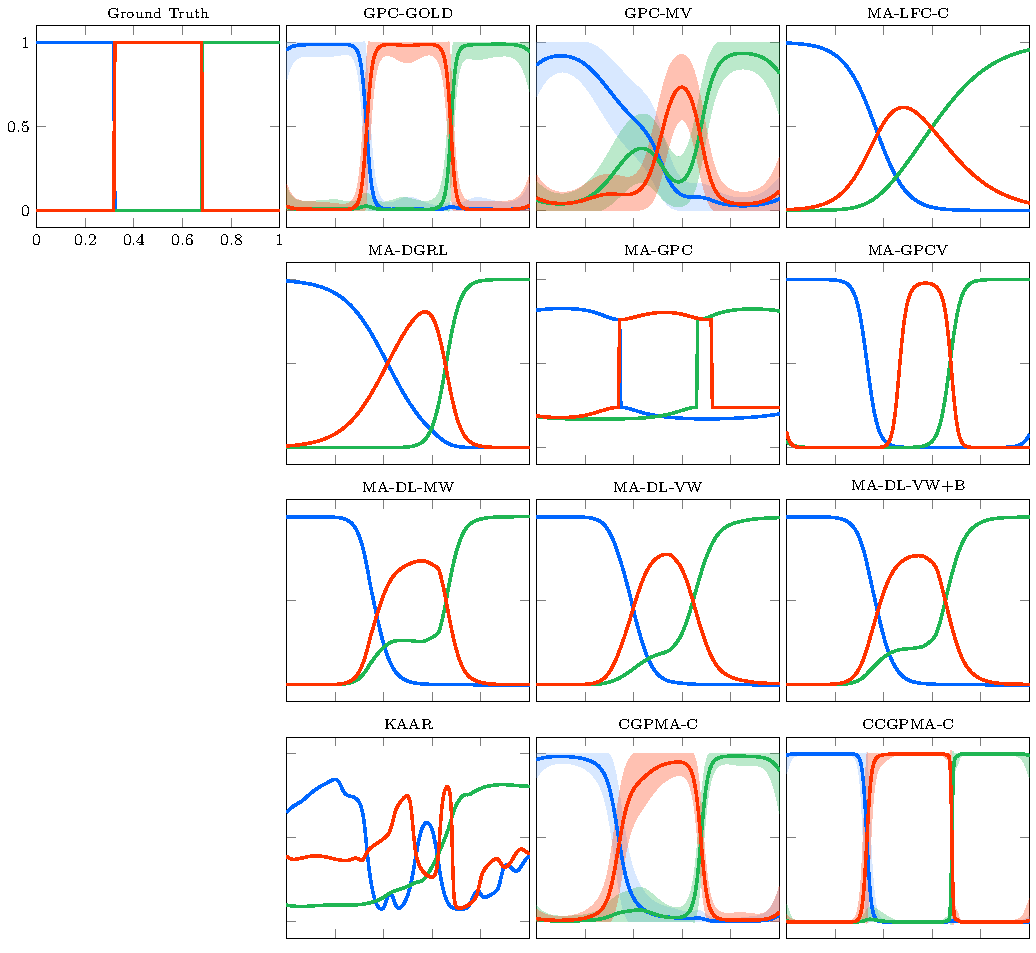
\includegraphics[width = 0.90\textwidth]{Figures/SinCla.pdf}
	\caption{Predicted mean label value for Fully synthetic dataset results. We compare the prediction of our CCGPMA-C($AUC=1$), and CCGPMA-C($AUC=0.9999$) with the theoretical upper bound GPC-GOLD($AUC=1.0$) and lower bound GPC-MV($AUC=0.9809$), and state-of-the-art approaches, MA-LFC-C($AUC=0.9993$), MA-DGRL($AUC=0.9999$),  MA-GPC($AUC=0.9977$), MA-GPCV($AUC=0.9515$), MA-DL-MW($AUC=0.9989$), MA-DL-VW($AUC=0.9972$), MA-DL-VW+B($AUC=0.9994$), KAAR($0.9099$). Note that the shaded region in GPC-MV, CGPMA-C, and CCGPMA-C indicates the area enclosed by the mean plus or minus two standard deviations. We remark that there is no shaded region for the rest of approaches since they do not provide information about the prediction uncertainty.}
	\label{fig:FSCla}
\end{figure*}
\begin{align}
\mat{W}=\begin{bmatrix}
0.4  &  0.7   & -0.5 &  0.0  & -0.7\\
0.4   &  -1.0  & -0.1  &  -0.8 & 1.0\\
3.1   &  -1.8  & -0.6  &  -1.2   & 1.0
\end{bmatrix},
\label{eq:parametersPC}
\end{align}
holding elements $w_{l_r,q}$. \cref{fig:FSCla} shows the predictive performance for all approaches for the \textit{fully synthetic} data. First, we highlight that the predicted mean label value--(PMLV) for KAAR, MA-GPC, and MA-GPCV presents a different shape compared with the ground truth; moreover, KAAR and MA-GPCV exhibit the worst AUC, even worse than the intuitive lower bound GPC-MV. We explain such conduct in the sense that these approaches are designed to deal with binary labels \cite{gil2018learning,rodrigues2014gaussian,ruiz2019learning}, while this dataset configures a 3-class classification problem. To face such a problem, we use the \textit{one-vs-all} scheme, which is not the most suitable alternative because, among other aspects, it leads to regions of input space that are ambiguously classified \cite{bishop2006pattern}. On the other hand, concerning MA-DL methods and the linear approaches MA-LFC-C and MA-DGRL, we note an akin predictive AUC; however, the linear approaches exhibit PMLV less similar to the Ground truth, which is due to MA-LFC-C and MA-DGRL only can deal with linearly separable data. Next, we analyze the results of our CCGPM-C and its particular case CCGPM-C. We remark that the predictive AUC of our methods is pretty close to the deep learning and linear models; however, unlike them, our CGPMA-C and CCGPMA-C show the most accurate PMLV compared with the absolute gold standard. In fact, CCGPMA-C behaves quite similar to GPC-GOLD, which is the theoretical upper bound. Finally, from the GPC-MV, we do not identify notably differences with the rest of the approaches (excluding KAAR and MA-GPCV), indicating that this first experiment seems not to be difficult.\\
\begin{figure*}[!tb]
	\centering
	%\input{Figures/VarEXp.tex}
	\includegraphics[width = 0.8\textwidth]{Figures/VarEXpC.pdf}
	\caption{Estimated reliabilities for the five annotators in the fully synthetic data. In the first column, from top to bottom, we expose the true reliabilities $\lambda_r$ used to simulate the labels from each annotator. The subsequent columns from top to bottom present the estimation of such reliabilities performed by state-of-the-art models that include these kinds of parameters in their formulation, where true values are provided in dashed lines. The shaded region in CGPMA-C and CCGPMA-C indicates the area enclosed by the mean plus or minus two standard deviations. Finally, we remark that the accuracy (Acc) is provided.}
	\label{fig:ExpCla}
\end{figure*}
From the above, we recognize that analyzing both the predictive AUC and the PMLV; our CCGPMA-C exhibits the best performance obtaining similar results compared with the intuitive upper bound (GPC-GOLD). Accordingly, we note CCGPMA-C proffers a more suitable representation of the labelers' behavior than its competitors because CCGPMA-C is the unique approach that models both the dependencies among the annotators and the relationship between the input features and the annotators' performance. To empirically support the above statement, \cref{fig:ExpCla} shows the estimated per-annotator reliability, where we only take into account models that include such types of parameters (MA-DGRL, CGPMA, and CCGPMA). From these results (visual inspection and the accuracy score) we note that the approach MA-DGRL (see column 2 in \cref{fig:ExpCla}) does not offer a proper representation of the annotators' behavior, which is a consequence of this model not considering the relationship between the input features and the labelers' decisions. On the other hand, our approaches CGPMA-C and CCGPMA-C (columns 3 and 4 in \cref{fig:ExpCla}) outperforms MA-DGRL, which is a direct repercussion of modeling the labelers' parameters as functions of the input features, which leads to a better representation of the labelers' behavior. We observe that CCGPMA-C exhibits the best performance in terms of accuracy; such an outcome is due to this method improves the quality of the annotators' model by considering correlations among the labelers (as was empirically established in \cite{zhu2019unsupervised,gil2018learning}).

\subsubsection{Semi-synthetic data results}
\begin{table*}[!htb]
	\centering
	%\tiny
	\scriptsize 
	\caption{Regression results in terms of AUC score over \textit{semi synthetic datasets}. Bold: the highest AUC excluding the upper bound GPC-GOLD.}
	\resizebox{.98\linewidth}{!}{
	\begin{tabular}{cccccccccc}\toprule
		{Method} & Breast & Bupa & Ionosphere & Pima & TicTacToe & Western & Wine & Segmentation & {Average}\\\midrule
		GPC-GOLD($M=40$)&$0.9907\pm0.0045$ & $0.6975\pm0.0466$ & $0.9490\pm0.0235$ & $0.8378\pm0.0302$ & $0.8429\pm0.0334$ & $0.9185\pm0.0061$ &$0.9987\pm0.0015$& $0.9596\pm0.0196$& $0.8993$\\ 
        GPC-GOLD($M=80$)&$0.9903\pm0.0046$ & $0.6997\pm0.0483$ & $0.9513\pm0.0225$ & $0.8374\pm0.0297$ & $0.8491\pm0.0323$ & $0.9250\pm0.0057$ &$0.9988\pm0.0016$& $0.9781\pm0.0041$& $0.9037$\\ 
        GPC-MV($M=40$)  &$0.9897\pm0.0045$ & $0.5366\pm0.0516$ & $0.7566\pm0.0572$ & $0.5399\pm0.0760$ & $0.6620\pm0.0357$ & $0.8658\pm0.0331$ &$0.8179\pm0.0212$& $0.9562\pm0.0228$& $0.7656$\\ 
        GPC-MV($M=80$)  &$0.9892\pm0.0048$ & $0.5698\pm0.0529$ & $0.7779\pm0.0550$ & $0.5302\pm0.0674$ & $0.6744\pm0.0357$ & $0.8446\pm0.0089$ &$0.8323\pm0.0487$& $0.9749\pm0.0047$& $0.7742$\\ 
        MA-LFC-C        &$0.8789\pm0.0510$ & $0.4593\pm0.1444$ & $0.7358\pm0.0901$ & $0.8119\pm0.0313$ & $0.6004\pm0.0261$ & $0.8400\pm0.0211$ &$0.9692\pm0.0357$& $0.9892\pm0.0031$& $0.7856$\\ 
        MA-DGRL         &$0.9757\pm0.0189$ & $0.5724\pm0.0336$ & $0.6453\pm0.0721$ & $0.8138\pm0.0290$ & $0.6129\pm0.0230$ & $0.8143\pm0.0150$ &$0.9795\pm0.0221$& $0.9897\pm0.0038$& $0.8005$\\ 
        MA-GPC          &$0.9811\pm0.0116$ & $0.5446\pm0.0578$ & $0.6631\pm0.1474$ & $0.5325\pm0.1780$ & $0.6079\pm0.0995$ & $0.8671\pm0.0114$ &$0.9417\pm0.0262$& $0.9734\pm0.0035$& $0.7639$\\ 
        MA-GPCV         &$0.8270\pm0.0547$ & $0.5567\pm0.0683$ & $0.6238\pm0.0871$ & $0.6217\pm0.0590$ & $0.6104\pm0.1003$ & $0.8451\pm0.0147$ &$0.9735\pm0.0172$& $0.9924\pm0.0027$& $0.7563$\\ 
        MA-DL-MW        &$0.9470\pm0.0173$ & $0.5237\pm0.0568$ & $0.7535\pm0.0543$ & $0.6178\pm0.0267$ & $0.6827\pm0.0296$ & $0.9092\pm0.0056$ &$0.9728\pm0.0109$& $0.9950\pm0.0017$& $0.8002$\\ 
        MA-DL-VW        &$0.9526\pm0.0245$ & $0.5327\pm0.0618$ & $0.6987\pm0.0497$ & $0.6063\pm0.0336$ & $0.6771\pm0.0267$ & $0.9173\pm0.0067$ &$0.9807\pm0.0152$& $\mathbf{0.9972\pm0.0011}$& $0.7953$\\ 
        MA-DL-VW+B      &$0.9465\pm0.0242$ & $0.5281\pm0.0631$ & $0.7196\pm0.0453$ & $0.6123\pm0.0378$ & $0.6780\pm0.0342$ & $0.9164\pm0.0085$ &$0.9817\pm0.0155$& $\mathbf{0.9972\pm0.0009}$& $0.7975$\\ 
        KAAR            &$0.8058\pm0.0274$ & $0.5920\pm0.0663$ & $0.7046\pm0.0739$ & $0.5802\pm0.0406$ & $0.6381\pm0.0545$ & $0.8588\pm0.0120$ &$0.9943\pm0.0105$& $0.9217\pm0.0190$& $0.7619$\\ 
        CGPMA-C($M=40$) &$0.9920\pm0.0038$ & $0.5537\pm0.0630$ & $0.8356\pm0.1002$ & $0.8201\pm0.0314$ & $0.7056\pm0.0304$ & $0.9178\pm0.0066$ &$0.9969\pm0.0028$& $0.9679\pm0.0065$& $0.8487$\\ 
        CGPMA-C($M=80$) &$0.9914\pm0.0038$ & $0.5945\pm0.0642$ & $0.8615\pm0.0696$ & $\mathbf{0.8204\pm0.0318}$ & $0.7048\pm0.0312$ & $0.9185\pm0.0057$ &$\mathbf{0.9986\pm0.0016}$& $0.9406\pm0.0061$& $0.8538$\\ 
        CCGPMA-C($M=40$)&$\mathbf{0.9938\pm0.0027}$ & $0.5734\pm0.0533$ & $0.9021\pm0.1079$ & $0.7810\pm0.0622$ & $\mathbf{0.7495\pm0.0539}$ & $0.9269\pm0.0058$ &$0.9952\pm0.0040$& $0.9774\pm0.0048$& $0.8624$\\ 
        CCGPMA-C($M=80$)&$0.9933\pm0.0030$ & $\mathbf{0.6022\pm0.0487}$ & $\mathbf{0.9023\pm0.1066}$ & $0.8045\pm0.0510$ & $0.7312\pm0.0323$ & $\mathbf{0.9307\pm0.0049}$ &$0.9955\pm0.0039$& $0.9774\pm0.0045$& $\mathbf{0.8671}$\\\bottomrule
	\end{tabular}}
	\label{tab:SSClaResults}
\end{table*}
We recall that for this type of data we have features from real-world problems whilst the data from multiple annotators were simulated as for \textit{fully synthetic data} (see \cref{eq:u1c,eq:u2c,eq:u3c,eq:parametersPC}). \cref{tab:SSClaResults} shows the results concerning this second experiment, where we highlight that the annotators were simulated by considering correlations among the labelers' opinions and modeling dependencies between such opinions and the input features. From \cref{tab:SSClaResults}, we can elucidate that, on average, our CCGPMA-C accomplishes the best predictive AUC; moreover, we note that CGPMA-C reaches the second-best performance in terms of AUC. Regarding the GPs-based competitors (GPC-MV, MA-GPC, MA-GPCV, and KAAR), we note that they offer the worst predictive performance in terms of AUC. The performance of MA-GPCV is expected because it represents the most naive method to deal with multi-labelers scenarios, which can be considered the theoretical lower bound. Conversely, analysing the results from MA-GPC, MA-GPCV, and KAAR, we note that they perform worse than MA-GPCV. We explain such an outcome in two regards. First, these approaches do not model the relationship between the input features and the annotators' performance, which does not fit how this experiment was conducted. Second, as we commented in the previous experiment, we use \textit{one-vs-all} scheme aiming to adapt these models for multi-class problems, which could be problematic as we have demonstrated in \cref{fig:ExpCla}; the above can be confirmed in the results for the multi-class datasets ``Western'' ($K=4$), ``Wine'' ($K=3$), and ``Segmentation'' ($K=10$), where the predictive AUC is lower compared with the remaining approaches. Then, analyzing the results from the DL-based approaches, we note a slightly better performance compared with the GPs-based methods (excluding CGPMA-C and CCGPMA-C). We argue that such an outcome is caused by the fact that DL models can handle both binary and multi-class classification problems; however, these DL models perform considerable worse that our proposal, which is due to CrowdLayer provide a very simple codification of the labelers' performance to guarantee a low computational cost \cite{morales2019scalable1}. Finally, from the linear models, we first analyze the outstanding, performance from MA-DGRL, which defeats all its non-linear competitors, and obtains a performance similar to the DL-based approaches. Initially, one can think that such an outcome is anomalous because a linear model is overcoming non-linear models; however, we argue that this is due to that the process of generating the labels from multiple annotators (see \cref{sec:datasets}) is similar to the labelers' model followed by MA-DGRL. On the other hand, regarding MA-LFC-C, we note a performance similar to the DL-based methods. Still, it is considerably lower than our proposal, which is due to that MA-LFC-C formulation is based on the assumption that the annotators' behavior is homogeneous across the input space, which does not correspond to the labels simulation procedure.   

\subsubsection{fully real data}
Finally, we use the \emph{fully real datasets}, which configure the most challenging scenario, due to both the input features and the labels from multiple labelers come from real-world applications.\\
\cref{tab:FSClaResults} outlines the achieved predictive AUC. First, we observe that for the voice data, the scales G and R exhibit a similar performance for all considered approaches; in fact, we highlight that GPC-MV obtains a performance comparable with the upper bound GPC-GOLD. The latter can be explained in the sense that for these scales, the annotators exhibit a suitable performance (i.e., the provided labels are similar to the ground truth). On the other hand, a reduction in the predictive AUC is observed for scale B, which is a consequence of a diminution in the labelers' performance compared with scales G and R, as demonstrated in \cite{gonzalez2015automatic}. We highlight that our approaches exhibit the best generalization performances for the three scales in the voice dataset. Remarkably, we note that CGPMA-C and CCGPMA-C do not suffer significant changes in the scale B, which is an outstanding outcome because it reflects that our approach offers a better representation of the labelers’ behavior even if the labels' quality decreases.

Finally, we review the results from the Music dataset. We note that our CCGPMA-C reaches the best predictive AUC; in fact, we highlight CCGPMA-C is the unique approach with performance comparable with the intuitive upper bound. We elucidate that such outstanding performance is due to that our approach improves the annotators' representation since it models dependencies among the labelers and computes the parameters of such model (related to the annotators' performance) as a function of the input features. On the other hand, we note a considerably low performance for MA-GPC, even lower than their intuitive lower bound (GPC-MV). This behavior has been a constant in the experiments; we argue that this outcome is because the Music dataset configures a multi-class classification problem, and we use a one-vs-all scheme for all of the binary classification (including MA-GP). Hence, as we have explained, such a scheme is not the most appropriate for multi-class problems.

\begin{table}[!htb]
	\centering
	%\tiny
	\scriptsize 
	\caption{Fully real datasets results. Bold: the method with the highest performance excluding the upper bound (target) classifier GPC-GOLD.}
	\resizebox{.98\linewidth}{!}{
	\begin{tabular}{cccccc}\toprule
		\multirow{2}{*}{Method}& \multicolumn{3}{c}{Voice} & \multirow{2}{*}{Music} & \multirow{2}{*}{Average}\\ & G & R & B &&\\\midrule
		GPC-GOLD($M=40$)&$0.9481$ & $0.9481$ & $0.9481$ & $0.9358$ & $0.9450$\\ 
        GPC-GOLD($M=80$)&$0.9484$ & $0.9484$ & $0.9484$ & $0.9178$ & $0.9407$\\ 
        GPC-MV($M=40$)  &$0.8942$ & $0.9373$ & $0.8001$ & $0.8871$ & $0.8797$\\ 
        GPC-MV($M=80$)  &$0.9301$ & $0.9377$ & $0.7962$ & $0.8897$ & $0.8884$\\ 
        MA-LFC-C        &$0.9122$ & $0.9130$ & $0.8406$ & $0.8599$ & $0.8814$\\ 
        MA-DGRL         &$0.9127$ & $0.9164$ & $0.8259$ & $0.8832$ & $0.8845$\\ 
        MA-GPC          &$0.8660$ & $0.8597$ & $0.4489$ & $0.8253$ & $0.7500$\\ 
        MA-GPCV         &$0.9283$ & $0.9208$ & $0.8835$ & $0.8677$ & $0.9001$\\ 
        MA-DL-MW        &$0.8957$ & $0.8966$ & $0.8123$ & $0.8567$ & $0.8653$\\ 
        MA-DL-VW        &$0.8942$ & $0.8929$ & $0.8092$ & $0.9167$ & $0.8782$\\ 
        MA-DL-VW+B      &$0.9030$ & $0.8937$ & $0.8218$ & $0.8573$ & $0.8689$\\ 
        KAAR            &$0.9109$ & $0.9351$ & $0.8969$ & $0.8896$ & $0.9081$\\ 
        CGPMA-C($M=40$) &$\mathbf{0.9324}$ & $0.9406$ & $0.8696$ & $0.9025$ & $0.9113$\\ 
        CGPMA-C($M=80$) &$\mathbf{0.9324}$ & $0.9417$ & $0.8708$ & $0.8987$ & $0.9109$\\ 
        CCGPMA-C($M=40$)&$0.9318$ & $\mathbf{0.9422}$ & $\mathbf{0.9002}$ & $0.9446$ & $\mathbf{0.9297}$\\ 
        CCGPMA-C($M=80$)&$0.9243$ & $0.9383$ & $0.8907$ & $\mathbf{0.9456}$ & $0.9247$\\ \bottomrule
	\end{tabular}}
	\label{tab:FSClaResults}
\end{table}

\subsection{Regression}

\subsubsection{fully real data}
Finally, we use the \textit{fully real datasets}, which present the most challenging scenario, where both the input samples and the labels come from real-world applications. 
\begin{table}[!htb]
	\centering
	%\tiny
	\scriptsize 
	\caption{Regression results in terms of $R^2$ score over \textit{fully real dataset}. Bold: the highest $R^2$ excluding the upper bound GPR-GOLD.}
	\resizebox{.45\linewidth}{!}{
	\begin{tabular}{cc}\toprule
		{Method} & {Music}\\\midrule
		GPR-GOLD($M=40$)&$0.4704$\\
        GPR-GOLD($M=80$)&$0.4889$\\
        GPR-Av($M=40$)  &$0.2572$\\
        GPR-Av($M=80$)  &$0.2744$\\
        MA-LFCR         &$0.1404$\\
        MA-GPR          &$0.0090$\\
        MA-DL-B         &$0.2339$\\
        MA-DL-S         &$0.2934$\\
        MA-DL-B+S       &$0.3519$\\
        CGPMA-R($M=40$) &$0.3345$\\
        CGPMA-R($M=80$) &$0.3531$\\
        CCGPMA-R($M=40$)&$0.3337$\\
        CCGPMA-R($M=80$)&$\mathbf{0.3872}$\\\bottomrule
	\end{tabular}}
	\label{tab:FSRegResults}
\end{table}
\cref{tab:FSRegResults} outlines the achieved performances. We remark that our CCGPMA-R with $M=80$ obtains the best generalization performance in terms of $R^2$ score. Further, as theoretically expected, its performance lies between that of GPR-GOLD and GP-Av. 
Moreover, regarding the GPs-based competitors (MA-GPR and CGPMA-R), we note that similarly to previous experiments, our CGPMA-R is just a bit lower than CCGPMA-R, which is due to both frameworks estimate the annotators' performances as functions of the input features. On the other hand, MA-GPR exhibits the worst prediction capability with a $R^2$ close to zero. We suppose the above is a symptom of overfitting, which can be confirmed due to the training $R^2$ score for MA-GPR is $0.4731$, which is comparable with GPR-GOLD. Conversely, the linear approach MA-LFCR exhibits the second-lowest performance and performs worse than the theoretical lower bound GP-Av, which indicates a non-linear structure in the Music dataset. Finally, analyzing the results from the deep learning approaches, we note that the variation MA-DL-B+S exhibit a similar performance compared with our CGPMA-R; however, it is slightly lower than than our CCGPMA-R. We highlight that despite the capacities of deep learning, our approach CCGPMA-R offers a better representation of annotators' behavior, unlike the deep learning approaches, which measure such performance using a single parameter.\\
On the other hand, we observe that all regression models presented a lower generalization performance than previous results (see \cref{tab:FSClaResults}) over the same dataset. The above is a repercussion of solving a multi-class classification problem with regression models.

\section{Conclusion}
We have introduced a Gaussian Process model suitable to deal with the problem of Multiple Annotators, named CCGPMA. Our CCGPMA is based on the correlated chained GP, which is a extension of the chained GP \cite{saul2016chained} introducing a semi-parametric latent factor model-(SLFM) to exploit correlations between the GP latent functions that model the parameters of a given likelihood function. Thereby, applying the CCGP to multiple annotators scenarios (CCGPMA), we are modeling the annotators' expertise as a functions of the input data and considering correlations among the labelers' answers. \\
We emphasize that to the best of our knowledge, CCGPMA is the first attempt to build a probabilistic framework that models the annotators' behavior by considering dependencies among the labelers and computing the annotators' performance as a function of the input features. Besides, we highlight that our approach can be used with different types of likelihood, which allows us to deal with both real-valued (regression) and categorical data (classification).\\ 
We tested our approach for regression and classification and using different scenarios regarding if the labels' were simulated (synthetic, semi-synthetic) or if they come from a real-world application (real-world dataset). Attained to the results, we remark that the CCGPMA can achieve robust predictive properties for both regression and classification scenarios. In fact, in most cases, our approach outperforms the models considered in this work for comparison. 

As future work, we believe that our work could be extended by using convolution processes \cite{alvarez2011computationally} instead of the SLFM, aiming to obtain a better representation of the correlations among the labelers. On the other hand, our approach could be extended to a context of multi-output Gaussian processes with multiple annotators, where for each output, we do not have access to an absolute ground truth but to a set of labels provided by multiple annotators. 

% use section* for acknowledgment
\section*{Acknowledgment}
Under grants provided by the Minciencias project: "Desarrollo de un prototipo funcional para el monitoreo no intrusivo de veh\'iculos
usando data analitycs para innnovar en el proceso de mantenimiento basado en la condici\'on en empresas de transporte p\'ublico."-code 643885271399. Julian Gil-Gonzalez is funded by the program ``Doctorados Nacionales - Convocatoria 785 de 2017''. MAA has been financed by the EPSRC Research Projects EP/R034303/1 and EP/T00343X/1. MAA has also been supported by the Rosetrees Trust (ref: A2501).


\bibliographystyle{IEEEtran}
\footnotesize
\bibliography{refs}
\vspace{-1.0cm}
\begin{IEEEbiographynophoto}{J. Gil-Gonzalez}
received his undergraduate degree in electronic engineering (2014) from the Universidad Tecnoloǵica de Pereira, Colombia. His M.Sc. in electrical engineering (2016) from the same university. Currently, he is PhD student from the same university. His research interests include probabilistic models for machine learning, learning from crowds, and Bayesian inference.
\end{IEEEbiographynophoto}
\vspace{-1.0cm}
\begin{IEEEbiographynophoto}{J. Giraldo}
received his undergraduate degree in electronic engineering (2014) from the Universidad Tecnoloǵica de Pereira, Colombia. His M.Sc. in electrical engineering (2016) from the same university. Currently, he is PhD student from the same university. His research interests include probabilistic models for machine learning, learning from crowds, and Bayesian inference.
\end{IEEEbiographynophoto}
\vspace{-1.0cm}
\begin{IEEEbiographynophoto}{A. Álvarez-Meza}
received his undergraduate degree in electronic engineering (2009), his M.Sc. degree in engineering industrial automation (2011), and his Ph.D. in engineering – automatics from the Universidad Nacional de Colombia. Currently, he is a Professor in the Department of Electrical, Electronic and Computation Engineering at the Universidad Nacional de Colombia at Manizales. His research interests include machine learning and signal processing.
\end{IEEEbiographynophoto}
\vspace{-1.0cm}
\begin{IEEEbiographynophoto}{A. Orozco-Gutierrez}
received his undergraduate degree in electrical engineering (1985) and his M.Sc. degree in electrical engineering (2004) from Universidad Tecnoloǵica de Pereira, and his Ph.D. in bioengineering (2009) from Universidad Politecnica de Valencia (Spain). He received his undergraduate degree in law (1996) from Universidad Libre de Colombia. Currently, he is a Professor in the Department of Electrical Engineering at the Universidad Tecnologica de Pereira. His research interests include machine learning and bioengineering.
\end{IEEEbiographynophoto}
\vspace{-1.0cm}
\begin{IEEEbiographynophoto}{M. A. Álvarez}
received the BEng degree in electronics engineering from the Universidad Nacional de Colombia (2004), the M.Sc. degree
in electrical engineering from the Universidad Tecnologica de Pereira, Colombia (2006), and the PhD degree in computer science from The University of Manchester, United Kingdom (2011). Currently, he is a Lecturer of Machine Learning in the Department of Computer Science, University of Sheffield, United Kingdom. His research interests include probabilistic models, kernel methods, and stochastic processes.
\end{IEEEbiographynophoto}









% Can use something like this to put references on a page
% by themselves when using endfloat and the captionsoff option.
% \ifCLASSOPTIONcaptionsoff
%   \newpage
% \fi



% trigger a \newpage just before the given reference
% number - used to balance the columns on the last page
% adjust value as needed - may need to be readjusted if
% the document is modified later
%\IEEEtriggeratref{8}
% The "triggered" command can be changed if desired:
%\IEEEtriggercmd{\enlargethispage{-5in}}

% references section

% can use a bibliography generated by BibTeX as a .bbl file
% BibTeX documentation can be easily obtained at:
% http://mirror.ctan.org/biblio/bibtex/contrib/doc/
% The IEEEtran BibTeX style support page is at:
% http://www.michaelshell.org/tex/ieeetran/bibtex/
%\bibliographystyle{IEEEtran}
% argument is your BibTeX string definitions and bibliography database(s)
%\bibliography{IEEEabrv,../bib/paper}
%
% <OR> manually copy in the resultant .bbl file
% set second argument of \begin to the number of references
% (used to reserve space for the reference number labels box)
\appendices
\crefalias{section}{appendix}
% \section{Related work}\label{RW}
% \cref{tab:SOA} summarizes the similarities and differences among our CCGPMA, and state-of-the-art approaches.
% \begin{table*}[!tb]
% 	\centering
% 	\caption{Survey of relevant supervised learning models devoted to multiple annotators.}
% 	\resizebox{1\linewidth}{!}{
% 		\begin{tabular}{C{5cm}cC{4cm}cC{3cm}cC{3cm}cC{3cm}}\toprule
% 			Source && Data type && Modeling the annotator’s expertise && Expertise as a function of the input space && Modeling the annotators' interdependencies 
%             \\\midrule
%             \textit{Raykar et al., 2010} \cite{raykar2010learning} && Regression-Binary-Categorical && \cmark && \xmark && \xmark\\
%             \textit{Zhang and Obradovic, 2011} \cite{zhang2011learning} && Binary && \cmark && \cmark && \xmark\\
%             \textit{Xiao et al., 2013} \cite{xiao2013learning} && Regression && \cmark && \cmark && \xmark\\
%             \textit{Yan et al., 2014} \cite{yan2014learning} && Binary && \cmark && \cmark && \xmark\\
%             \textit{Wang and Bi, 2016} \cite{wang2016bi}&& Binary && \cmark && \cmark && \xmark\\
%             \textit{Rodrigues et al., 2017} \cite{rodrigues2017learning} && Regression-Binary-Categorical && \cmark && \xmark && \xmark\\
%             \textit{Gil-Gonzalez et al., 2018} \cite{gil2018learning} && Binary && \cmark && \xmark && \cmark\\
%             \textit{Hua et al., 2018} \cite{hua2018collaborative} && Binary-Categorical && \cmark && \xmark && \xmark\\
%             \textit{Ruiz et al., 2019} \cite{ruiz2019learning} && Binary && \cmark && \xmark && \xmark\\
%             \textit{Morales- ́Alvarez et al., 2019} \cite{morales2019scalable} && Binary && \cmark && \xmark && \xmark\\
%             \textit{Zhu et al., 2019} \cite{zhu2019unsupervised} && Regression && \cmark && \xmark && \cmark\\
%             % \textbf{Proposal-(CGPMA)} && Regression-Binary-Categorical && \cmark && \cmark && \xmark\\
%             \textbf{Proposal-(CCGPMA)} && Regression-Binary-Categorical && \cmark && \cmark && \cmark\\\bottomrule
% 	\end{tabular}} 
% 	\label{tab:SOA}
% \end{table*}

\section{Approximate inference for the CCGP model}\label{ApInCCGP}
The actual posterior can be approximated by a parametrized variational distribution $p(\hat{\ve{f}},{\ve{u}}|\mat{Y})\s{\approx} q(\hat{\ve{f}},{\ve{u}})$, as:
\begin{align}
\label{eq:VarCCGP}
q(\hat{\ve{f}}, {\ve{u}}) = p(\hat{\ve{f}}|{\ve{u}})q({\ve{u}})= \prod_{j=1}^{J}p(\ve{f}_j|{\ve{u}})\prod_{q=1}^{Q}q(\ve{u}_q),
\end{align}
where $p(\ve{f}_j|{\ve{u}})$ is given by \cref{eq:CCGPprior}, $q(\ve{u}_q)\igual\gauss(\ve{u}_q|\ve{m}_q,\mat{V}_q)$, and $q({\ve{u}})\igual \gauss({\ve{u}}|\ve{m},\mat{V})$. Also, $\ve{m}_q\en\Real^{M}$, and $\mat{V}_q\en \Real^{M\times M}$ are respectively the mean and covariance of variational distribution $q(\ve{u}_q)$; similarly, $\ve{m} \igual [\ve{m}_1^{\top}, \dots , \ve{m}_Q^{\top}]^{\top}\en \Real^{QM}$, and $\mat{V}\en \Real^{QM\times QM}$ is a block-diagonal matrix with blocks given by the covariance matrices $\mat{V}_q$. We remark that the variational approximation given by \cref{eq:VarCCGP} is not uncommon, and it has been used in several GPs models, including \cite{saul2016chained,moreno2018heterogeneous}.\\
Accordingly, the approximation for the posterior distribution comprises the computation of the following variational parameters: the mean vectors $\{\ve{m}_q\}_{q=1}^{Q}$ and the covariance matrices $\{\mat{V}_q\}_{q=1}^{Q}$. Such an estimation is carried out by maximizing an evidence lower bound--(ELBO), which is given as:
\begin{align}
\mathcal{L}
=&\sum_{n=1}^{N}\mathbb{E}_{\prod\limits^J_{j=1}q(\ve{f}_1),\dots , q(\ve{f}_J)}\left[\log p(y_n|\theta_1(\ve{x}_n),\dots , \theta_J(\ve{x}_n))\right]-\cdots\nonumber\\
&\cdots-\sum_{q=1}^{Q} \mathbb{D}_{KL}(q(\ve{u}_q)||p(\ve{u}_q))\label{eq:LowBound21},
\end{align}
where $\mathbb{D}_{KL}(\cdot||\cdot)$ is the Kullback-Leibler divergence and $q(\ve{f}_j)$ is defined as follows:
\begin{align}
\notag q(\ve{f}_j) &=\gauss(\ve{f}_j|\mat{K}_{\ve{f}_j\ve{u}}\mat{K}_{\ve{u}\ve{u}}^{-1}\ve{m}, \mat{K}_{\ve{f}_j\ve{f}_j}+\cdots\\
& \cdots + \mat{K}_{\ve{f}_j\ve{u}}\mat{K}_{\ve{u}\ve{u}}^{-1}(\mat{V}-\mat{K}_{\ve{u}\ve{u}})\mat{K}_{\ve{u}\ve{u}}^{-1}\mat{K}_{\ve{u}\ve{f}_j}).
\end{align}
Yet, in presence of non-Gaussian likelihoods, the computation of the variational expectations in \cref{eq:LowBound21} cannot be solved analytically~\cite{saul2016chained,moreno2018heterogeneous}. Therefore, aiming to model different data types, i.e., classification and regression tasks, we need to find a generic alternative to solve the integrals related to these expectations. In that sense, we use the Gaussian-Hermite quadratures approach as in~\cite{hensman2015scalable,saul2016chained}.\\
It is worth mentioning that the CCGPs objective functions exhibit an ELBOW that allows Stochastic Variational Inference--(SVI)~\cite{blei2017variational}. Hence, the optimization is solved through a \textit{mini-batch}-based approach from noisy estimates of the global objective gradient, which allows dealing with large scale datasets~\cite{hensman2015scalable,saul2016chained,moreno2018heterogeneous}. The ELBO is optimized to estimate the variational parameters $\left\{\ve{m}_q, \mat{V}_q\right\}_{q=1}^{Q}$. Besides, such an ELBO can be used to infer the model's hyperparameters such as the inducing points location, the kernel hyperparameters, and the combination factors $w_{j,q}$ associated with the LFs in \cref{eq:SLFM}.


\section{CCGPMA applied for regression tasks}\label{CCGPMAReg}
For real-valued outputs, e.g., $\mathcal{Y} \s{\subset}\Real$, we follow the multi-annotator model used in \cite{raykar2010learning,groot2011learning,xiao2013learning,rodrigues2017learning}, where each output $y_n^r$ is a corrupted version of the hidden ground truth $y_n$. Then, the likelihood function is given as:
\begin{align}
\label{eq:RegLik}
p(\mat{Y}|{\bm{\theta}}) = \prod^N_{n=1}\prod_{r\in R_n}\gauss\left(y_n^r|y_n,v_{n}^r\right),
\end{align}
where $v_{n}^r\en\Real^+$ is the $r$-th annotator error-variance for the instance $n$. In turn, to model this likelihood function with CCGPMA, it is necessary to chain each likelihood's paramater to a latent function $f_j$. Thus, we require $J\igual R+1$ LFs; one to model the hidden ground truth, such that $y_n\igual f_1(\ve{x}_n)$, and $R$ LFs to model each of the error-variances $v_{n}^r\igual \exp(f_{l_r}(\ve{x}_n))$, with $r\en \left\{1, \dots R\right\}$, and $l_r = r+1 \in \left\{2, \dots J\right\}$. Note that we use an exponential function to code $f_{l_r}$ and $v_{n}^r$, aiming to guarantee $v_{n}^r\s{>}0$ ($f_{l_r}\en \Real$).

\subsection{Datasets and simulated/provided annotations}\label{dataReg}
To control the label generation~\cite{ruiz2019learning}, we build \textit{semi-synthetic data} from six datasets related to regression tasks from the well-known {UCI repository}. We selected the following datasets: {Auto MPG Data Set}--(Auto), {Bike Sharing Dataset Data Set}--(Bike), {Concrete Compressive Strength Data Set}--(Concrete), {The Boston Housing Dataset}--(Housing),\footnote{See https://www.cs.toronto.edu/$\sim${d}elve/data/boston/bostonDetail.html for housing} {Yacht Hydrodynamics Data Set}--(Yacht), and {Relative location of CT slices on axial axis Data Set}--(CT).  
Third, we evaluate our proposal on one \textit{fully real dataset}, we use the Music dataset introduced in0\cref{sec:datasets}. Notice that the music dataset configures a 10-class classification problem; however in this first experiment we are using our CCGPMA with a likelihood function designed for real-valued labels \cref{eq:RegLik}. Such practice is not uncommon in machine learning, and it is usually known as ``Least-square classification'' \cite{rasmussen2006gaussian}. \cref{tab:RegData} summarizes the tested datasets for the regression case.
\begin{table}[!tb]
	\caption{Datasets for regression.
	}
	\label{tab:RegData}
	\centering
	\resizebox{\linewidth}{!}{
		\begin{tabular}{ccccC{2cm}cC{2cm}}\toprule
			&& Name && Number of features && Number of instances\\\midrule
		\multirow{ 1}{*}{\textit{fully synthetic}}	&& synthetic && 1 && 100\\\midrule
		\multirow{ 6}{*}{\textit{semi-synthetic}}   && Auto&& 8 && 398\\ 
		                                            && Bike && 13 && 17389\\
		                                            && Concrete && 9 && 1030\\
		                                            && Housing && 13 && 506\\
		                                            && Yacht && 6 && 308\\
		                                            && CT && 384&&53500
		                                            \\\midrule
      	\multirow{ 1}{*}{\textit{fully real}}       && Music && 124 && 1000
      	\\\bottomrule
	\end{tabular}}
\end{table}
As we pointed out previously, \textit{fully synthetic} and \textit{semi-synthetic} datasets do not hold real annotations. Thus, it is necessary to generate these labels synthetically as a version of the gold standard corrupted by Gaussian noise, i.e., $y_n^r = y_n +\epsilon^r_{n}$, where $\epsilon^r_{n}\sim \gauss(0, v^r_{n})$, being $v^r_{n}$ the $r$-th annotator error-variance for the sample $n$. Note that we are interested in interested in modelling such an error-variance for the $r$-th annotator as a function of the input features, which is correlated with the variances of the other labelers. For doing so, the error variances are generated as follows:
\begin{itemize}
    \item Define $Q$ functions $\mu_q(\cdot)$, and the combination parameters $w_{l_r,q},\,\forall r, q$.
    \item For each annotator $r$ and sample $n$, compute $f_{l_r,n} = \sum_{q=1}^{Q}w_{l_r,q}\mu_q(\hat{x}_n)$, where $\hat{x}_n$ is the $n$-th component of $\hat{\ve{x}}\in \Real$, which is an $1-$D representation of input features $\mat{X}$ by using the t-distributed Stochastic Neighbor Embedding approach \cite{maaten2008visualizing}.
    \item Finally, determine $v^r_n = \exp(f_{l_r,n})$. 
\end{itemize}
\subsection{Method comparison and performance metrics}
\begin{table}[bt!]
	\caption{A brief overview of state-of-the-art methods tested for regression tasks. GPR: Gaussian Processes Regression, LR: logistic regression, Av: average, MA: multiple annotators, DL: Deep learning, LFCR: Learning from crowds for regression.
	}
	\label{tab:RegVal}
	\centering
	\resizebox{1\linewidth}{!}{
		\begin{tabular}{lcl}\toprule
			Algorithm && Description \\\midrule
			GPR-GOLD  && A GPR using the real labels (upper bound).\\
			GPR-Av    &&  A GPR using the average of the labels as the ground truth.\\
			MA-LFCR~\cite{raykar2010learning}  && A LR model for MA where the labelers' parameters\\
			&& are supposed to be constant across the input space.\\
			%MA-LMO~\cite{xiao2013learning}   && A multi-labeler approach where\\
			%&&the sources parameters depend on the input space.\\
			MA-GPR~\cite{rodrigues2014gaussian}	 &&  A multi-labeler GPR, which is as an extension of MA-LFCR.\\
			MA-DL~\cite{rodrigues2018deep}  && A Crowd Layer for DL, where the annotators' parameters\\
			&&  are constant across the input space.\\
			CGPMA-R  &&  A particular case of our CCGPMA for regression,\\
    		&& where $Q=J$, and $w_{j,q}\igual 1$ if $j\igual q,$ otherwise $w_{j,q}\igual 0.$\\\bottomrule
	\end{tabular}}
\end{table}
The quality assessment is carried out by estimating the regression performance as the coefficient of determination--($R^2$). A cross-validation scheme is employed with 15 repetitions where $70$\% of the samples are utilized for training and the remaining $30\%$ for testing (except for \textit{fully synthetic dataset}, since it clearly defines the training and testing sets). \cref{tab:RegVal} displays the employed methods of the state-of-the-art for comparison purposes. From \cref{tab:RegVal}, we highlight that for the model MA-DL, the authors provided three different annotators' codification: MA-DL-B, where the bias for the annotators is measured; MA-DL-S, where the labelers' scale is computed; and measured; MA-DL-B+S, which is a version with both \cite{rodrigues2018deep}. 
\subsection{Results over semi-synthetic data}
We perform a controlled experiment aiming to verify the capability of our CCGPMA to estimate the performance of inconsistent annotators as a function of the input space and taking into account their dependencies. For this first experiment, we use the \textit{semi-synthetic} dataset described in \cref{dataReg}. We simulate five labelers ($R=5$) with different levels of expertise. To simulate the error-variances, we define $Q=3$ functions $\mu_q(\cdot)$, which are given as 
\begin{align}
\label{eq:u1r}
\notag \mu_1(x) &= 4.5\cos(2\pi x + 1.5\pi) - 3\sin(4.3\pi x + 0.3\pi) +\cdots\\ & \cdots + 4\cos(7\pi x + 2.4\pi),\\
\label{eq:u2r}
\notag \mu_2(x) &= 4.5\cos(1.5\pi x + 0.5\pi) + 5\sin(3\pi x + 1.5\pi) - \cdots\\ & \cdots - 4.5\cos(8\pi x+ 0.25\pi),\\
\label{eq:u3r}
\mu_3(x) &= 1,
\end{align}
where $x\in [0,1]$. Besides, we define the following combination matrix $\mat{W} \in \Real^{Q\times R}$, where
\begin{align}
\mat{W}=\begin{bmatrix}
-0.10  &  0.01   & -0.05 &  0.01  & -0.01\\
0.10   &  -0.01  & 0.01  &  -0.05 & 0.05\\
-2.3   &  -1.77  & 0.54  &  0.9   & 1.42
\end{bmatrix},
\label{eq:parametersP}
\end{align}
holding elements $w_{l_r,q}$. 
\begin{table*}[!b]
	\centering
	%\tiny
	\scriptsize 
	\caption{Regression results in terms of $R^2$ score over \textit{semi synthetic datasets}. Bold: the highest $R^2$ excluding the upper bound GPR-GOLD.}
	\resizebox{.98\linewidth}{!}{
	\begin{tabular}{cccccccc}\toprule
		{Method} & {Auto} & {Bike} & {Concrete} & {Housing} & {Yacht} & {CT} & {Average}\\\midrule
		GPR-GOLD($M=40$)&$0.8604\pm0.0271$ & $0.5529\pm0.0065$ & $0.8037\pm0.0254$ & $0.8235\pm0.0419$ & $0.8354\pm0.0412$ & $0.8569\pm0.0055$ & $0.7888$\\ 
        GPR-GOLD($M=80$)&$0.8612\pm0.0279$ & $0.5603\pm0.0063$ & $0.8271\pm0.0230$ & $0.8275\pm0.0399$ & $0.8087\pm0.0423$ & $0.8648\pm0.0047$ & $0.7916$\\ 
        GPR-Av($M=40$)  &$0.8425\pm0.0286$ & $0.5280\pm0.0100$ & $0.7589\pm0.0279$ & $0.7834\pm0.0463$ & $0.7588\pm0.0498$ & $0.8070\pm0.0130$ & $0.7464$\\ 
        GPR-Av($M=80$)  &$0.8406\pm0.0304$ & $0.5397\pm0.0085$ & $0.7765\pm0.0274$ & $0.7903\pm0.0451$ & $0.7676\pm0.0535$ & $0.8167\pm0.0089$ & $0.7552$\\ 
        MA-LFCR         &$0.7973\pm0.0218$ & $0.3385\pm0.0051$ & $0.6064\pm0.0384$ & $0.7122\pm0.0509$ & $0.6403\pm0.0186$ & $\mathbf{0.8400\pm0.0014}$ & $0.6558$\\ 
        MA-GPR          &$0.8456\pm0.0281$ & $0.4448\pm0.0187$ & $0.7769\pm0.0367$ & $0.7685\pm0.0632$ & $0.7842\pm0.1027$ & $0.0105\pm0.0045$ & $0.6051$\\
        MA-DL-B         &$0.7766\pm0.0253$ & $0.5854\pm0.0107$ & $0.2319\pm0.0328$ & $0.5317\pm0.1005$ & $0.2089\pm0.0783$ & $0.6903\pm0.2689$ & $0.5041$\\ 
        MA-DL-S         &$0.7761\pm0.0279$ & $\mathbf{0.5828\pm0.0149}$ & $0.2363\pm0.0252$ & $0.5352\pm0.0948$ & $0.1822\pm0.0985$ & $0.9394\pm0.0257$ & $0.5420$\\ 
        MA-DL-B+S       &$0.7717\pm0.0239$ & $0.5816\pm0.0181$ & $0.2369\pm0.0322$ & $0.5330\pm0.0850$ & $0.1974\pm0.0895$ & $0.5517\pm0.2316$ & $0.4787$\\ 
        CGPMA-R($M=40$) &$0.8474\pm0.0221$ & $0.5464\pm0.0069$ & $0.8169\pm0.0231$ & $0.7946\pm0.0498$ & $0.7545\pm0.1029$ & $0.8236\pm0.0132$ & $0.7639$\\ 
        CGPMA-R($M=80$) &$0.7768\pm0.0708$ & $0.5560\pm0.0074$ & $0.8190\pm0.0254$ & $0.8058\pm0.0493$ & $0.8230\pm0.0760$ & $0.8371\pm0.0104$ & $0.7696$\\ 
        CCGPMA-R($M=40$)&$0.8563\pm0.0247$ & $0.5284\pm0.0117$ & $0.7976\pm0.0270$ & $0.7994\pm0.0462$ & $0.8436\pm0.0507$ & $0.8219\pm0.0062$ & $0.7745$\\ 
        CCGPMA-R($M=80$)&$\mathbf{0.8578\pm0.0244}$ & $0.5467\pm0.0069$ & $\mathbf{0.8220\pm0.0259}$ & $\mathbf{0.8110\pm0.0453}$ & $\mathbf{0.8476\pm0.0544}$ & $0.8252\pm0.0083$ & $\mathbf{0.7850}$\\\bottomrule
	\end{tabular}}
	\label{tab:SSRegResults}
\end{table*}
\cref{tab:SSRegResults} shows the results the experiment with \textit{semi synthetic dataset}. On average, our CCGPMA-R  exhibits the best generalization performance in terms of the $R^2$ score. On the other hand, regarding its GPs-based competitors (GPR-Av, MA-GPR, and CGPMA-R), we first note that the performance of CGPMA-R exhibit a similar (but lower) performance than CCGPMA-R. The above is a consequence of that conversely to CGPMA-R our CCGPMA-R model the annotators' interdependencies. Secondly, the intuitive lower bound GPR-Av exhibits a significantly worse prediction than our approaches. On the other hand, we remark the behavior of MA-GPR, which is lowest compared with its GPs-based competitors, even far worse than the supposed lower bound GPR-Av. The key to this abnormal outcome lies in the formulation of this approach; MA-GPR models the annotators' behavior by assuming that their performance does not depend on the input features and considering that the labelers make their decisions independently, which does fit the process that we use to simulate the labels for this experiment.
Next, we analyze the results concerning the linear model MA-LFR; attained to the results, we note that this approach's prediction capacity is far lower than our approaches; the above outcome suggests that there may exist a non-linear structure in most databases. However, we highlight a particular result for the dataset CT, where MA-LFCR exhibits the best performance defeating all its competitors based on non-linear models. From the above, we intuit that the CT dataset may have a linear structure. To confirm this supposition, we perform an additional experiment over CT by training a regression scheme based on LR with the actual labels (we follow the same scheme as for GPR-GOLD). We obtain an $R^2$ score equal to $0.8541$ (on average), which is close to the results obtained by GPR-GOLD. Thus, we can elucidate that there exists a linear structure in the dataset CT. Finally, we analyze the results for the DL-based models. Similar to the experiments over \textit{fully synthetic datasets}, we note a considerable low prediction capacity; in fact, they are even defeated by the linear model MA-LFR. Again, we attribute this behavior to the fact that the CrowdLayer (used to manage the data from multiple annotators) does not offer a suitable codification of the labelers' behavior. Nevertheless, taking the above into account, we observe an unusual result in the dataset Bike, where the DL-based approaches offer the best performance, even defeating the supposed upper-bound GPR-GOLD. To explain that, it is necessary to analyze the meaning of the target variable in such a dataset. Regarding to the description of this dataset,\footnote{Such description can be found in https://archive.ics.uci.edu/ml/datasets/bike+sharing+dataset} the target variables indicate the count of total rental bikes, including both casual and registered in a day. The above suggests that there may exist a quasi-periodic structure in the dataset, which cannot be captured by the GPR-GOLD since it uses a non-periodic kernel (it uses the RBF kernel). To support our suppositions, an additional experiment was performed over this dataset by training the model GPR-GOLD with the kernel defined as follows. 
\begin{align}\label{eq:Pkernel}
\kappa(\ve{x}_n, \ve{x}_{n^{\prime}}) = \varphi \exp \left[  - \frac{1}{2}\sum_{p=1}^{P}\left( \frac{\sin(\frac{\pi}{T_p} (x_{p,n}- x_{p,n^{\prime}}) )}{l_p}\right)^2 \right],
\end{align}
where $\varphi\in \Real$ is the variance parameter, $l_p\in (\Real^{+})$ is the length-scale parameter for the $p$-th dimension, and $T_p\in (\Real^{+})$ is the period for the $p$-th dimension. Therefore, we obtain an $R^2$ score equal to $0.5952$ (on average), which is greater than the obtained by the DL-based approaches, indicating a quasi-periodic structure in the Bike dataset as we had supposed.
% biography section
% 
% If you have an EPS/PDF photo (graphicx package needed) extra braces are
% needed around the contents of the optional argument to biography to prevent
% the LaTeX parser from getting confused when it sees the complicated
% \includegraphics command within an optional argument. (You could create
% your own custom macro containing the \includegraphics command to make things
% simpler here.)
%\begin{IEEEbiography}[{\includegraphics[width=1in,height=1.25in,clip,keepaspectratio]{mshell}}]{Michael Shell}
% or if you just want to reserve a space for a photo:

% \begin{IEEEbiography}{Michael Shell}
% Biography text here.
% \end{IEEEbiography}
% % if you will not have a photo at all:


% insert where needed to balance the two columns on the last page with
% biographies
%\newpage

% \begin{IEEEbiographynophoto}{Jane Doe}
% Biography text here.
% \end{IEEEbiographynophoto}

% You can push biographies down or up by placing
% a \vfill before or after them. The appropriate
% use of \vfill depends on what kind of text is
% on the last page and whether or not the columns
% are being equalized.

%\vfill

% Can be used to pull up biographies so that the bottom of the last one
% is flush with the other column.
%\enlargethispage{-5in}



% that's all folks
\end{document}


